\documentclass{uflamon}          % classe base para a monografia

%==============================================================================
% Utilizacao de pacotes
\usepackage[T1]{fontenc}         % usa fontes postscript com acentos
\usepackage[brazil]{babel}       % hifenização e títulos em português do Brasil
\usepackage[utf8]{inputenc}     % permite edição direta com acentos
\usepackage{amsmath}             % pacote da AMS para Matemática Avançada
\usepackage{amssymb}             % símbolos extras da AMS
\usepackage{latexsym}            % símbolos extras do LaTeX
\usepackage{graphicx}            % para inserção de gráficos
\usepackage{listings}            % para inserção de código
\usepackage{fancyvrb}            % para inserção de saídas de comandos
%\usepackage{enumerate}           % para personalizar lista enumeradas 

											%(incluso na classe)
\usepackage{longtable}           % para tambelas muito grandes NOVO!!!!

\usepackage{colortbl} % cores em tabelas
\newcolumntype{Z}{|>{\columncolor[gray]{0.9}}l|} %cor cinza em células
%\usepackage{array} % já incluso na classe
\newcolumntype{L}[1]{>{\raggedright\let\newline\\\arraybackslash\hspace{0pt}}m{#1}}
\newcolumntype{C}[1]{>{\centering\let\newline\\\arraybackslash\hspace{0pt}}m{#1}}
\newcolumntype{R}[1]{>{\raggedleft\let\newline\\\arraybackslash\hspace{0pt}}m{#1}}
\usepackage{multirow} % para juntar duas linhas em uma só

\usepackage{multicol} % para uso de várias colunas

% cores para os links cruzados
\usepackage{color}
\definecolor{rltred}{rgb}{0.2,0,0}
\definecolor{rltgreen}{rgb}{0,0.2,0}
\definecolor{rltblue}{rgb}{0,0,0.2}

\usepackage[colorlinks=true,
            urlcolor=rltblue,       % \href{...}{...} external (URL)
            filecolor=rltgreen,     % \href{...} local file
            linkcolor=rltred,       % \ref{...} and \pageref{...}
            citecolor=rltgreen,
            pdftitle={Exemplo de Uso da Classe Uflamon},
          pdfauthor={Joaquim Quinteiro Uchôa},
          pdfsubject={Este texto tem por objetivo servir de exemplo da classe Uflamon.},
          pdfkeywords={Comunicação Científica. 2. Pesquisa . 3. Pesquisa Científica. 
 					 4. Redação. 5. Monografia.}%
]{hyperref} % para referência cruzadas
%\usepackage{hyperref}            % para referência cruzadas
\usepackage{subfigure}           % figuras dentro de figuras
\usepackage{caption}            % remodelando o formato dos títulos de 
                                 % tabelas e figuras

% configuração padrão do listings   
\lstset{
   language=Java,
   extendedchars=true,
   tabsize=3,
   basicstyle=\footnotesize\ttfamily,
   stringstyle=\em,
   showstringspaces=false 
}

% para referências de acordo com a ABNT
% precisa instalar o abntex2 antes!!!
% http://abntex.codigolivre.org.br/
% comente se pretende usar outro padrão

%abnt-emphasize=bf coloca o título das bibliografias em negrito
%abnt-thesis-year=both
\usepackage[alf,abnt-etal-cite=3,abnt-etal-list=3,abnt-url-package=url,abnt-emphasize=bf]{abntex2cite}

% evite usar o hyperref com abntex, pode dar caca em urls... no linha anterior, informo
% para incluir urls usando o pacote url e não o hyperref
%
% caso queira o hyperref com abntex, comente a linha anterior e descomente a seguinte
%\usepackage[alf,abnt-etal-cite=3,abnt-etal-list=0,abnt-etal-text=emph]{abntex2cite}
%
% caso vc ainda use a versão anterior da abntex, comente a linha incluindo o abntex2cite
% e descomente a próxima linha 
%\usepackage[alf,abnt-etal-cite=3,abnt-etal-list=0,abnt-etal-text=emph]{abntcite}


% redefinindo formatação de títulos de tabelas e figuras


%==============================================================================
% para os fãs do Word, descomente as linhas abaixo
%\sloppy %mais espaço entre as linhas
%\usepackage{identfirst} %identando-se a primeira linha de cada seção
%\noindentfirst % Tire o comentário para manter o padrão do LaTeX.

%==============================================================================
% definido comandos na monografia - não é necessário na sua monografia 
% apenas para exemplificar a definição de novos comandos
\newcommand{\defs}[1]{\textsl{#1}}


% Especificando hifenizações que por ventura LaTeX não saiba fazer
% Por padrão 99,9% dos termos em português devem ser hifenizados corretamente.
\hyphenation{hardware software Li-nux am-bien-te diag-nos-ti-car coor-de-na-ção 
FAE-PE Recovery TelEduc Williams UFLA}

%==============================================================================
% Dados da monografia, capa: autor, titulo, banca, etc... - SUBSTITUA DE ACORDO
%==============================================================================
\author{Mallu Eduarda Batista}
\title{Módulo WEB para o Diário de Classe}
\subtitle{Uma implementação voltada às necessidades do professor}
\engtitle{}
\engsubtitle{}
\edicao{}
\date{}
\tipo{Relatório Técnico apresentada à Universidade Federal de Lavras, como parte das exigências para a obtenção do título de Bacharel em Ciência da Computação.}
% use \orientador ou \orientadora quando for o caso
\orientadora{Prof. Dra. Ana Paula Piovesan Melchiori}
%\orientadora{}
% use \coorientador ou \coorientadora quando for o caso
%coorientadora{} % comente se não tiver coorientador
%\coorientador{}
\local{Lavras -- MG}
\bancaum{Profa. Dra. Renata Teles Moreira}{UFLA}
% \bancadois{Prof. DSc. João Banca Dois}{FCO} % comente se sua banca tiver só um professor
\bancadois{Prof. Dr. José Monserrat Neto}{UFLA}
% \bancadois{Prof. DSc. João Banca Dois}{FCO} % comente se sua banca tiver só um professor
\bancatres{Karla Emanuella Veloso Pinto}{Prefeitura Municipal de Lavras}
% \bancaquatro{Prof. Esp. Carlos Banca Quatro}{IBGPLUS}
\defesa{31 de janeiro de 2018}
%==============================================================================
%##################################################
% Dados para Ficha catalográfica, gerada pelo sistema da Biblioteca da UFLA
% http://www.biblioteca.ufla.br/FichaCatalografica/
% dados para ficha catalográfica
% Elaboração da Ficha Catalográfica
%\preparofichacat{Ficha catalográfica elaborada pela Coordenadoria de Processos Técnicos \\ da Biblioteca Universitária da UFLA}
% primeiro autor - como na primeira linha da ficha catalográfica
%\fcautor{Batista, Mallu Eduarda}
% autores, separados por vírgula - na ficha catalográfica, no formato que
% vem após o título e a barra ("/")
%\fcautores{Mallu Eduarda Batista}
% caso trabalho seja ilustrado (figuras, gráficos, tabelas, etc.), 
% então informar por meio do comando a seguir
% caso não seja ilustrado, basta comentá-lo
%\fcilustrado{il.}
% dados da edição para a ficha 
%\fcedicao{2$^a$ ed. rev., atual. e ampl.}
% tipo do trabalho (tese, dissertação, etc.), de acordo com sistema
% de geração de ficha catalográfica
%\fctipo{Relatório Tecnico (monografia)}
% ano da defesa, só precisa informar se for diferente do ano da publicação
% se forem iguais, comente a linha a seguir
% \fcdatadefesa{2018}
% preencher aqui com os dados de catalogação gerados pelo sistema
%\fccatalogacao{1. TCC. 2. Monografia. 3. Dissertação. 4. Tese. 5. Trabalho Científico – Normas. I. Universidade Federal de Lavras. II. Título.}
%\fcclasi{808.066}


%##################################################

%\antesfichacat{\noindent Para citar este documento: \\UNIVERSIDADE FEDERAL DE LAVRAS. Biblioteca Universitária. \textbf{Manual de normalização e estrutura de trabalhos acadêmicos: TCC, monografias, dissertações e teses}. 2. ed. rev., atual. e ampl. Lavras, 2015. Disponível em: \url{http://www.biblioteca.ufla.br/wordpress/wpcontent/uploads/bdtd/manual_normalizacao_UFLA.pdf}. Acesso em: data de acesso.}

%\depoisfichacat{\noindent A reprodução e a divulgação total ou parcial deste trabalho são autorizadas, por qualquer meio convencional ou eletrônico, para fins de estudo e pesquisa, desde que citada a fonte.\\
%\newline
%{\small Este documento possui páginas em branco para facilitar a impressão frente-e-verso.}}

%##################################################

%##################################################

% para os exemplos do manual
%\newenvironment{exemplomanual}{
%\vspace{0.5cm}
%\noindent\begin{minipage}{\textwidth}
%\noindent\rule{\textwidth}{0.5pt}
%\vspace{-1cm}
%\begin{flushleft}
%}{
%\end{flushleft}
%\vspace{-0.6cm}
%\noindent\rule{\textwidth}{0.5pt}
%\vspace{0.3cm}
%\end{minipage}
%}

%\newenvironment{exemplomanuallista}{
%\vspace{0.3cm}
%\noindent\begin{minipage}{\textwidth - 0.5cm}
%\noindent\rule{\textwidth}{0.5pt}
%\vspace{-1cm}
%\begin{flushleft}
%}{
%\end{flushleft}
%\vspace{-0.6cm}
%\noindent\rule{\textwidth}{0.5pt}
%\vspace{0.3cm}
%\end{minipage}
%}

% por conta de alguns exemplos
%\usepackage{setspace}

%##################################################

% se vc já defendeu e tem o arquivo escaneado da folha de rosto, 
% descomente e altere o nome do arquivo
%\folhaAprovacaoAssinada{folharosto}

% Aqui começa o documento propriamente dito
\begin{document}

\maketitle

\dedic{Para toda minha família e amigos. Em especial, para minha mãe Elizabete.}     % Dedicatórias\\


\thanks{
A Deus por me guiar e proteger por todos os caminhos.
	
Aos meus pais, pela educação, exemplo, apoio e força na realização desse sonho. Sem vocês nada disso seria possível ou teria sentido. 

A toda minha família, pela de união e parceria. Meus irmãos Marcello e Marcos Paulo, por mais que me esgotem, transmitem muito amor . Minha tia Eliete, pelos anos de companheirismo, exemplo admirável e principal incentivadora de buscar e ir atrás dos meus objetivos. Minhas tias Elaine e Eliz que sempre me apoiaram em tudo. Minha vovó Maria Néria por todo carinho e amor.

Aos meus amigos e amigas: Ana Laura, Arthur, Danielle, Débora, Luana,  Maria Fernanda, Nádia, Sanndy, Tatiane, pelo apoio nas mais diversas situações, presença nos melhores momentos, ombro nos piores e companheirismo sempre. Mas, principalmente por nunca desistirem de mim, apesar de tudo. 

Aos meus queridos e incríveis amigos que ganhei durante faculdade; Elder, Gabriel e Matheus (White), pela atenção, longas horas de paciência e aprendizado, amizade  e companheirismo durante essa jornada. Vocês foram essenciais na minha formação acadêmica e pessoal.  

As minhas amigas Giovana, Carol e Laura, por me acolherem em casa nessa reta final, proporcionarem muitas alegrias, risadas, concelhos, broncas e por se tornarem indispensáveis no meu dia.

A professora Dra. Ana Paula pelos anos de acolhida, orientação, aprendizado, companheirismo e amizade.

A Universidade Federal de Lavras, ao departamento de Ciência da Computação e seu corpo docente, pelo suporte e aprendizado durante esses anos.

}      
    % Agradecimentos

\epigrafe{ % citação opcional
Se as nossas vontades não coincidirem, que a Sua prevaleça. \\}

% palavras-chave
\palchaves{Diário de Classe. Professor. Módulo WEB. Ferramenta educacional. }
\resumo{
O diário de classe é um documento oficial escolar, para fins administrativos, e de inteira responsabilidade do professor. 
Este trabalho teve como objetivo a criação e implementação de um módulo WEB para o diário de classe, visando ser um ambiente onde os professores cadastrem e administrem diários e suas respectivas informações, em um único lugar.
O desenvolvimento foi feito usando a linguagem de programação PHP, padrão de arquitetura MVC, framework \textit{Bootstrap} e as tecnologias HTML5, CSS3, JavaScript e JQuery.
Como resultado, é disponibilizado a aplicação web para uso de professores, no âmbito de suas atribuiçoes agregando segurança, agilidade de armazenamento, e acesso á informação.
	}
	   % Resumo (digite aqui o resumo)

% keywords devem vir antes do abstract
\keywords{Class diary. Teaching. Technology. Educational tool.} % keywords
\abstract{The class diary is an official school document and the teacher's full responsibility.
	The objective of this work was to create and implement a WEB module for the class journal, aiming at an environment where teachers register and manage journals and their respective information, in a single place.
	The development was done using a PHP programming language, MVC architecture standard, framework Bootstrap and as HTML5, CSS3, JavaScript and JQuery technologies.
As a result, a web application is available for use by teachers, not its integrated assignments, storage agility and access to information.}

%##################################################

% Dados do guia
%\begin{titlepage}
%\pagestyle{empty}
%\renewcommand{\baselinestretch}{1}
%\enlargethispage{1.5cm}
%\input{reitoria}
%\cleardoublepage
%\end{titlepage}

%##################################################

% descomente para habilitar a lista desejada
\listoffigures                             % Lista de Figuras
%\listofilustracoes
%\listofgraficos							   % Lista de Gráficos
\listoftables                              % Lista de Tabelas
%\listofquadros							   % Lista de Quadros
%\listofexemplos
%\listofteoremas
\tableofcontents                           % Sumário

\clearpage

\pagestyle{ufla}

%==============================================================================
% incluindo os capitulos
\chapter{INTRODUÇÃO}
\label{cap:introducao}


A constante busca pela facilidade de acesso à informação, tem motivado cada vez mais o desenvolvimento de sistemas Web. Estes por sua vez, diferentemente do modelo tradicional, não precisam ser instalados e são acessíveis de qualquer lugar, por qualquer dispositivo conectado à internet. Atualmente, esse tipo de tecnologia é voltada para as mais diversas áreas e é empregada com várias finalidades, inclusive na educação.

No campo educacional, a gestão escolar retoma os conceitos de eficiência e melhoria no sistema de ensino, e é por meio dela que se busca organizar as áreas da escola. Nesse contexto, a adoção de sistemas para auxiliar a gestão escolar, automatizando o processo, traz benefícios como o aumento na produtividade dos funcionários, dados concretos e facilidade de acesso à informação. 


Muitas escolas da atual rede de ensino brasileira, ainda adotam a utilização do Diário de papel pelos professores. Esse, é o documento oficial no qual são registradas todas as atividades pedagógicas abordadas, bem como o histórico de presença e notas de cada aluno, e é posteriormente repassado à secretaria ao final de cada período letivo, através da entrega da taleta. Tal processo é manual, lento e passível de erros, o que caracteriza a necessidade da adoção de um sistema mais eficiente e seguro a fim de melhorar o processo de gestão dessas informações.



Tomando como ponto de partida o estudo "Diários de Classe: traços históricos de um ensino de língua" de Menegolo e Cardoso, que analisou a aplicação real desse material, concluiu-se que as anotações realizadas pelos professores não condizem com as aulas lecionadas, mas sim com uma cultura escolar predeterminada que visa suprir as cobranças de um sistema de ensino frágil. Tal omissão corrobora para dificultar um diagnóstico preciso e correto sobre as falhas educacionais e as áreas que carecem de mudança imediata. Nesse sentido, a utilização de ferramentas tecnológicas, como sistemas Web, tem sido modelados para auxiliar na busca de uma solução prática e segura na tentativa de amenizar tais problemas.



A busca por ferramentas para auxiliar no problema abordado, levou a criação de projetos como o Educação Conectada\footnote{http://www.educacaoconectada.com.br/}, que desenvolveu um aplicativo móvel para dispositivos Android\footnote{https://www.android.com/} que desempenha a mesma função do diário de papel supracitado. Entretanto foram identificados problemas na interface da aplicação, quanto as funcionalidades, e foram tratadas para melhor atender as necessidades do usuário final segundo padrões e técnicas de \textit{design} centrado no usuário, produzindo como resultado final, um novo protótipo de interface \cite{igor2016}. 


\section{Objetivos}


\subsection{Objetivo geral}

Este trabalho tem como objetivo geral desenvolver um sistema Web para o perfil do professor, que funcione como um Diário de Classe virtual, substituindo o Diário de papel. A interface da aplicação será baseada nos resultados obtidos por Lacerdino e Melchiori (2016).


\subsection{Objetivos Específicos}


Os objetivos específicos norteiam: 

\begin{itemize}
	\item Estudo das ferramentas necessárias para o desenvolvimento da aplicação;
	\item Especificação de requisitos: levantamento de requisitos, diagrama de casos de uso e protótipo de interface;
	\item Projeto do software: definição dos módulos e componentes, criação do banco de dados e padrão de arquitetura MVC;
	\item Implementação: codificação;
	\item Teste: dinâmico, com validação das funcionalidades através da interface (teste de caixa branca) durante a implementação;
	
\end{itemize}













\chapter{REFERENCIAL TEÓRICO}
\label{cap:referencial}

A Revolução da informação, tida como a terceira das maiores revoluções, é resultado da acelerada difusão das tecnologias da informação e comunicação (TICs). Com a modernização dos computadores e a instauração das Redes de Computadores, possibilitou o compartilhamento de recursos físicos e lógicos (\textit{e-maisl}, impressoras, entre outros) expandindo ainda mais a conexão entre tecnologia e pessoas \cite{helmano1995}.


O uso de computadores nas escolas, traduz o que pode-se chamar de pensamento crítico \cite{valente1993}. É através dele que se explica porque a utilização de tecnologia educacional transmite informações e corroba em serviços úteis à educação e a prática pedagógica, como por exemplo, promover o aprendizado de matemática por meio de jogos educacionais interativos em sala de aula \cite{seabra1993}.

Devido a essa modernização tecnológica, é notório que as organizações visam constantemente o alcance de processos de mudanças e inovações, em busca de qualidade e competitividade. Segundo Fonseca (2001), para alcançar esses objetivos, as empresas devem se preocupar com o envolvimento de seus colaboradores no processo produtivo/serviço, e consequentemente a qualidade de vida dos mesmos, o que envolve condições de trabalho, novas formas de gestão, saúde física e mental, entre outras. No entanto, ao analisar o sistema educacional, percebemos que o método de trabalho do professor ainda é estagnado, dificultando a efetividade e organização das funções cabíveis a eles.


Associar a tecnologia às práticas pedagógicas é um desafio a ser enfrentado: de um lado estão as ferramentas educacionais que tendem a facilitar as tarefas diárias e moderniza-las ao mesmo tempo, do outro, os professores, que alegam carecer de conhecimento frente a essas tecnologias \cite{REP's1158}. Logo, um dos meios de solucionar o problema é aderindo a substituição de ferramentas ultrapassadas utilizadas no processo educacional, a fim de facilitar o trabalho desses profissionais.

Como exemplo temos o Diário de Classe, descrito segundo o manual de orientação \cite{manualDiario} , “um instrumento de registro do planejamento e do desenvolvimento das atividades pedagógicas do(a) professor(a), instrumento legal de registro das situações didáticas da vida escolar dos(as) estudantes, do acompanhamento das suas aprendizagens e do desempenho escolar. No diário de classe devem constar: a relação nominal dos(as) estudantes, em ordem alfabética, observações sobre o rendimento, frequência justificada e atitudes comportamentais; o planejamento das aulas, o registro dos conteúdos trabalhados em situação didática de cada bimestre e as atividades ou projetos especiais.” . O diário é disponibilizado em forma de livro, onde o preenchimento deve ser feito manualmente e sem rasuras, sendo elas rubricadas e justificadas quando acontecido \cite{teresa1999manual}.


Nas escolas, exitem vários relatos da utilização de TICs, bem como sua viabilização e aceitação. Kasin e Silva (2008) relata como o computador e a \textit{Internet} tornam-se aliados no processo ensino-aprendizagem, integrando em sua metodologia softwares autorais para criação coletiva, quando o professor busca conhecimentos amplos na utilização de tecnologias educacionais, mediando todo o processo. Outro exemplo, é a utilização do Diário Escolar Digital, uma "plataforma idealizada pela Secretaria de Estado de Educação de MInas Gerais - SEEMG - e desenvolvida pela Prodemge, cuja proposta é ampliar a interação entre estudantes, pais, responsáveis e profissionais da educação (Professores, Especialistas, Diretores e Secretários de Escola)" segundo o site Escola Interativa.
 

Elas devem agir de forma a complementar o ensino tradicional, e jamais substituir a instituição principal; a escola. O professor por sua vez, deve incrementar em seu currículo e, simultaneamente em suas aulas, uma formação ampla para permear a difusão de conhecimento através da utilização dessas tecnologias  \cite{albino2016avaliaccao}. Sendo assim, tecnologias voltadas à educação tendem a complementar e modificar a prática pedagógica afim de surtirem  facilidades e modernização de ferramentas e métodos. Entretanto, é importante ressaltar que o professor é ferramenta primordial nesse processo.


Ponte (2002), afirma que " Na escola, as TIC são um elemento constituinte do ambiente de aprendizagem. Ou seja, é parte do sistema para acarretar benefícios. "[...]Representam, além disso, uma ferramenta de trabalho do professor e do educador de infância e um elemento integrante da sua cultura
profissional" \cite[p. 2]{ponte2002tic}. 



\chapter{MATERIAL E MÉTODOS}
\label{cap:desenvolvimento}

Os materiais e métodos descritos, contextualizam parte do desenvolvimento do sistema Web proposto.

\section{Ferramentas utilizadas}

Aqui são descritas as ferramentas utilizadas na implementação do código-fonte, interface, base de dados e algumas auxiliares.

\subsection{Interface gráfica}
A linguagem de marcação criada pelo físico britânico Tim Berners-Lee, se tornou a mais utilizada para a construção de páginas da Web \cite{doi:10.1080/02763869.2011.540212}. Após diversas reestruturações, em sua grande maioria realizadas pela \textit{World Wide Web Consortium} (W3C) , o HTML - \textit{HyperText Markup Language} (Linguagem de Marcação de Hipertexto) se encontra em sua quinta versão - HTML5.  Segundo \cite{curso2010html5} "Um dos principais objetivos do HTML5 é facilitar a manipulação do elemento possibilitando o
desenvolvedor a modificar as características dos objetos de forma não intrusiva e de maneira que
seja transparente para o usuário final."

\textit{Cascading Style Sheets} - CSS\footnote{www.css3.info/}  é utilizado para estilizar uma pagina, de forma a adicionar um \textit{link} direto para um documento que contém toda a formatação de estilo utilizada. Possui sintaxe simples, com termos em inglês e possibilita declaração de seletores em blocos.

Bootstrap\footnote{https://getbootstrap.com/} possibilita a criação de projetos responsivos e móveis, utilizando ferramentas de código aberto e componentes de \textit{front-end}. É voltado para o desenvolvimento com HTML, CSS, JS e utilização de \textit{plugins} criados no jQuery\footnote{https://jquery.com/}, além de disponibilizar uma extensa lista de componentes pré-construídos para uso \cite{spurlock2013bootstrap}.

\subsection{Base de dados}

MySQL WorkBench é um SGBD - Sistema Gerenciador de banco de dados, que fornece modelagem de dados e uso de SQL\footnote{ Linguagem de pesquisa declarativa padrão para banco de dados relacional (base de dados relacional)}   - \textit{Structured Query Language}, ou Linguagem de Consulta Estruturada. 

\subsection{Desenvolvimento das funcionalidades}

\textit{Model-View-Controller} - MVC é um padrão arquitetural formulado por Trygve Reenskaug em 1979, para definir quais são os elementos do software e como eles interagem entre si. Tal ferramenta busca proporcionar escalabilidade e eficiência da aplicação \cite{Karam2009SynchronousOH}.Seu principal benefício é isolar as regras de negócio da lógica de apresentação. Para reduzir o acoplamento e aumentar a coesão nas classes, três camadas propostas para serem independentes e podem ser descritas da seguinte maneira:

\begin{itemize}
	\item[]\qquad\textit{Model} ou modelo funciona como regras de negocio. Gerencia elementos de dados, responde requisições do controlador e efetua alterações de estado.
	\item[]\qquad\textit{View} ou visão, é responsável por apresentar informações ao usuário, recebendo instruções do controlador e informações do modelo.
	\item[]\qquad\textit{Controller} ou controlador, é o intermediador entre as requisições do usuário, passadas da visão para as regras de negócio e/ou o contrário. É o único que possui conhecimento dessas duas camadas.
\end{itemize}




PHP\footnote{http://www.php.net/} -\textit{ Hipertext Preprocessor}  é uma linguagem de \textit{script open source}, amplamente utilizada, adequada para o desenvolvimento web e que pode ser embutida dentro do HTML. Delimitada por \textit{tags} representando início e fim, permitindo alternar entre dentro e fora do "modo PHP" \cite{tonu2012php}.


JavaScript \footnote{https://www.javascript.com}  é uma linguagem de programação interpretada. Criada em 1995, tida como a principal linguagem de programação para navegadores web, que utilizam o modelo cliente servidor, multiparadigma, com tipagem dinâmica, fraca e implicite \cite{javaScript2011}.


\subsection{Ferramentas auxiliares}


Aqui abordadas, as ferramentas auxiliares no desenvolvimento do software, tem por objetivo manter o registro de alteração de dados e integrar outras ferramentas de desenvolvimento úteis em um único lugar. 

Git \footnote{https://git-scm.com/}  , pronuncia-se “git” ou “dit”, em inglês britânico é um sistema de controle de versão distribuído (livre e de código aberto), e um sistema de gerenciamento de código fonte com ênfase em velocidade e eficiência. Inicialmente foi projetado para desenvolvimento do Kernel Linux \footnote{Forma a estrutura base do sistema operacional/sistema operativo GNU/Linux, que é um sistema operacional tipo unix.}   mas teve sua adoção para diversos outros projetos  \cite{moreira2016desbravando}.

GitHub \footnote{https://github.com/}   é um serviço web que permite hospedar repositórios de projetos que utilizam Git . Assim ele facilita o trabalho em equipe e incentiva a  colaboração com projetos \textit{open source} \cite{moreira2016desbravando}.

NetBeans IDE\footnote{https://netbeans.org/}   é um ambiente de desenvolvimento integrado, gratuito e de código aberto. Voltado para desenvolvedores de softwares. Aceita as principais linguagens de programação atuais como JAVA, PHP, JavaScript, HTML5, entre outras \cite{tonu2012php}.




\chapter{DESENVOLVIMENTO DO SISTEMA}
\label{cap:sistema}	

Neste capítulo são abordadas as fases de desenvolvimento do software.

\section{Especificação de requisitos}


O módulo proposto visa satisfazer as necessidades do professor, quanto a utilização dos recursos do diário virtual. Isso impossibilita o compartilhamento de informações necessárias ao professor, como a lista de alunos por exemplo, que deveria ser fornecida por outro módulo (secretaria). Logo, a inserção desses dados fazem parte dos requisitos do sistema atual. Na Tabela \ref{tab:reqfuncionais} são descritos os requisitos funcionais levantados para o modo professor.


\begin{table}[h]
	
	\vspace{0.5cm}.
	\centering
	\begin{tabular}{lll}
		%coluna separa-se por &
		% \\ quebra de linha 
		% \hline para linha horizontal
		\hline	
		Identificador & Descrição \\
		\hline
		RF001 &	O software deve possibilitar adicionar um Diário \\
		RF002 &	O software deve possibilitar a visualização do Diário \\
		RF003 &	O software deve possibilitar a exclusão do Diário \\
		
		RF004 &	O software deve possibilitar a visualização dos Alunos\\
		RF005 &	O software deve possibilitar adicionar um novo Aluno\\
		RF006 &	O software deve possibilitar excluir Aluno\\
		RF007 &	O software deve possibilitar alterar Aluno\\
		
		RF008 &	O software deve possibilitar a visualização das Aulas\\
		RF009 &	O software deve possibilitar adicionar uma nova Aula\\
		RF010 &	O software deve possibilitar excluir Aula\\
		RF011 &	O software deve possibilitar alterar Aula\\
		
		RF012 &	O software deve possibilitar a visualização das Avaliaçãoes\\
		RF013 &	O software deve possibilitar adicionar uma nova Avaliação\\
		RF014 &	O software deve possibilitar excluir Avaliação\\
		RF015 &	O software deve possibilitar alterar Avaliação \\
		
		\hline
	\end{tabular}
	\caption{Requisitos funcionais}
	\label{tab:reqfuncionais}
\end{table}

Estes, foram traduzidos para um diagrama de caso de uso, que por sua vez tem a função de documentar o que o sistema faz, no ponto de vista do usuário. Ele pode ser observado na Figura \ref{fig:UseCaseDiagram0}; o professor, que é o único usuário do módulo, consegue realizar tarefas (casos de uso) no sistema, para cada diário que ele possuir.

\begin{figure}[!htb]
	\centering
	\caption{Diagrama de caso de uso} %legenda
	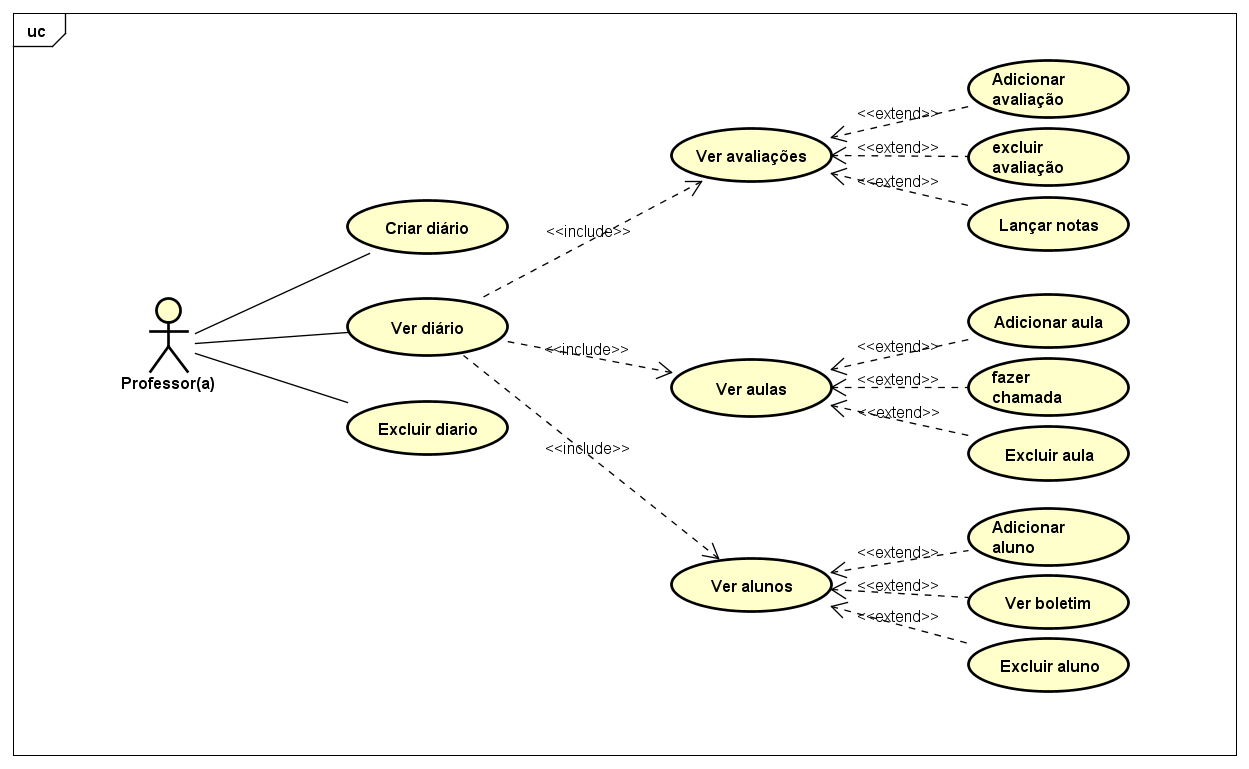
\includegraphics[scale=0.4]{UseCaseDiagram0}\\  % o 0.9 indica 90% do tamanho original
	% pdfLaTeX aceita figuras no formato PNG, JPG ou PDF
	% figuras vetoriais podem ser exportadas para eps e depois convertidas para pdf usando epstopdf
	{\small } %Fonte da imagem
	\label{fig:UseCaseDiagram0} %rotulo para refencia
\end{figure}




\section{Projeto}


O professor desempenha tarefas importantes com o uso do diário. São elas:

\begin{itemize}
	\item Efetuar o registro da aula, informando a data e um resumo geral específico sobre o conteúdo lecionado nesse dia.
	
	\item Registrar também qualquer ocorrência ou fato relevante que aconteça em sala de aula
	
	\item Realizar a chamada colocando "presença" ou "falta" para cada aluno matriculado na matéria referente a chamada.
	
	\item Transcrever as atividades avaliativas e informar o valor atribuído a cada uma delas, bem como a nota obtida por cada aluno nestas atividades.
	
	\item Fechar as notas de cada aluno ao final do período escolar, preenchendo a taleta (relatório).
	
	
\end{itemize}

Tais tarefas foram transcritas ao ambiente de desenvolvimento em formas de adaptações na produção da interface. 

O módulo permite que cada professor acesse o conteúdo de seus diários. Para isso, é preciso efetuar \textit{login} com \textit{e-mail} e senha, possibilitando a criação de um novo cadastro, caso ainda não possua. Dentro de cada diário estão disponíveis cadastro e acesso à alunos, avaliações e aulas. 



\subsection{Estruturação do banco de dados}

Após a definição dos principais requisitos do sistema e suas funcionalidades, foi estruturado uma base de dados para armazenar as informações necessárias para o funcionamento do módulo. Para isso, optou-se pelo modelo relacional, que possibilita criar entidades e o relacionamento entre elas.

As entidades modeladas (tabelas) representam as principais estruturas de dados necessárias para implementação das funcionalidades do sistema. São elas nomeadas de: Professor, Diário, Aluno, Avaliação, Nota, Chamada, Aula, PeriodoDeRegime e Turma. Tais nomes foram adotados,  sugestivamente, como abstração dos objetos do mundo real para facilitar o entendimento. Assim, podemos dizer por exemplo que, nesse sistema, dadas as necessidades, o Professor(representado pela tabela professor) possui atributos (dados) "nome, e-mail, senha e uma imagem de perfil".

A estrutura final das entidades e do relacionamento entre elas, é apresentado na Figura \ref{fig:relacional}. O script SQL (\textit{Structured Query Language}, ou Linguagem de Consulta Estruturada) exportado, é utilizado pelo servidor para criação e disponibilização ao banco de dados para uso na aplicação.  

\begin{figure}[!htb]
	\centering
	
	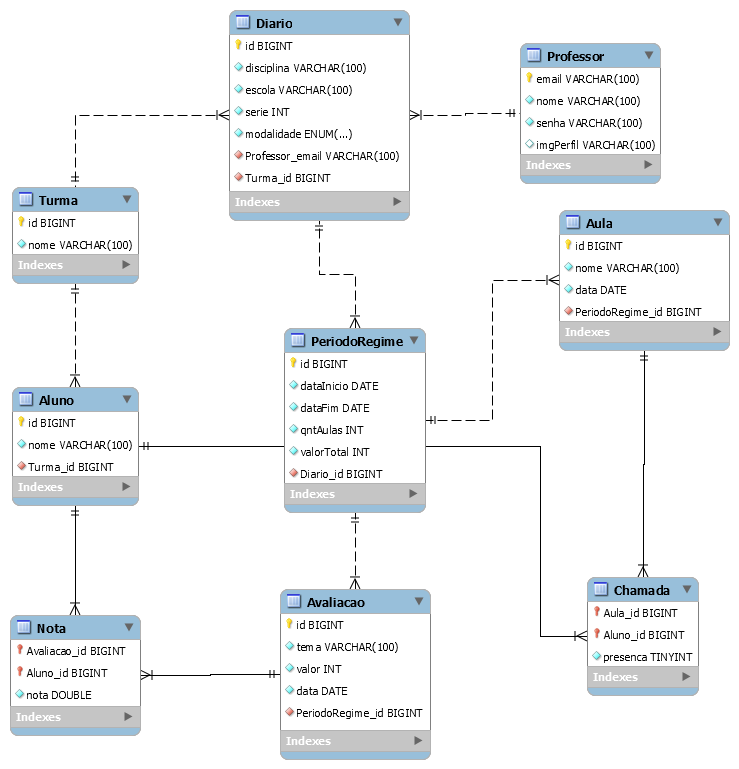
\includegraphics[scale=0.6]{relacional}\\  % o 
	\caption{Modelo relacional do banco de dados} %legenda
	{\small } %Fonte da imagem
	\label{fig:relacional} %rotulo para refencia
\end{figure}

\section{Implementação}


Para desenvolvimento do software, adotou-se o uso da arquitetura \textit{Model-view-controller} - MVC. Tal arquitetura propõe que seja feita a separação da representação da informação (dados), da interação do usuário (interface). A arquitetura da implementação do Diário de Classe encontra-se estruturada em três diretórios: \textit{Model}, \textit{View} e \textit{Controller}. Tal divisão com seus respectivos arquivos são mostrados na Figura \ref{fig:controller-model} e Figura \ref{fig:view}.

\begin{figure}[!htb]
	\centering
	
	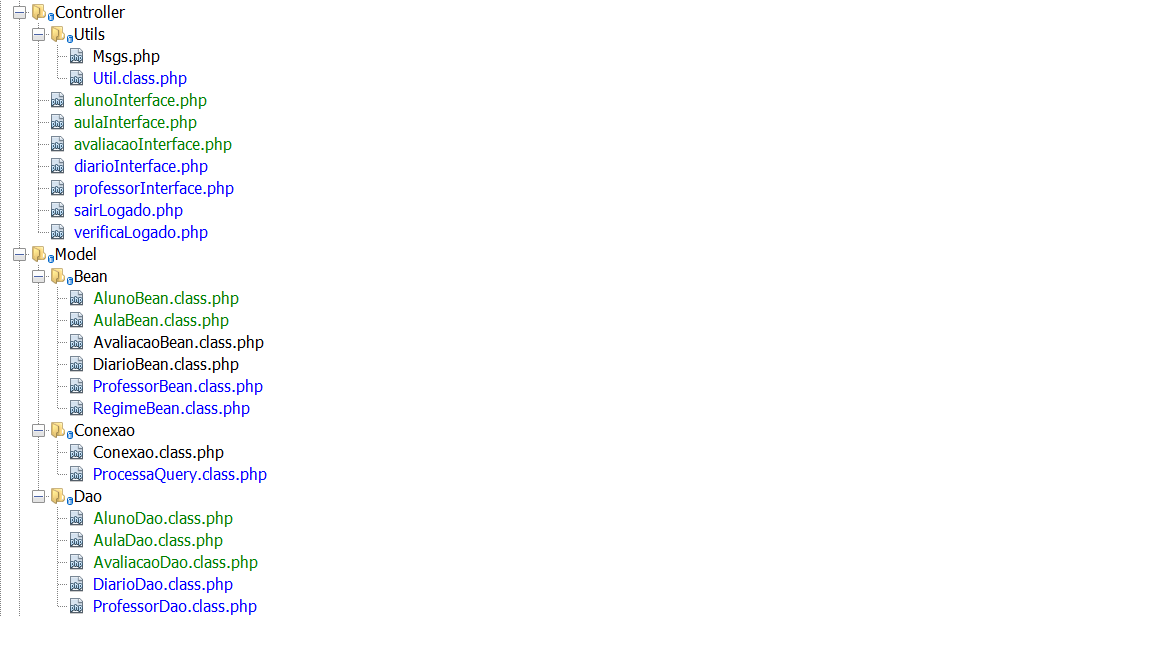
\includegraphics[scale=1.0]{controller-model}\\  % o 0.9 indica 90% do tamanho original
	% pdfLaTeX aceita figuras no formato PNG, JPG ou PDF
	% figuras vetoriais podem ser exportadas para eps e depois convertidas para pdf usando epstopdf
	\caption{Divisão dos diretórios - controller e model} %legenda
	{\small } %Fonte da imagem
	\label{fig:controller-model} %rotulo para refencia
\end{figure}

\begin{figure}[!htb]
	\centering	
	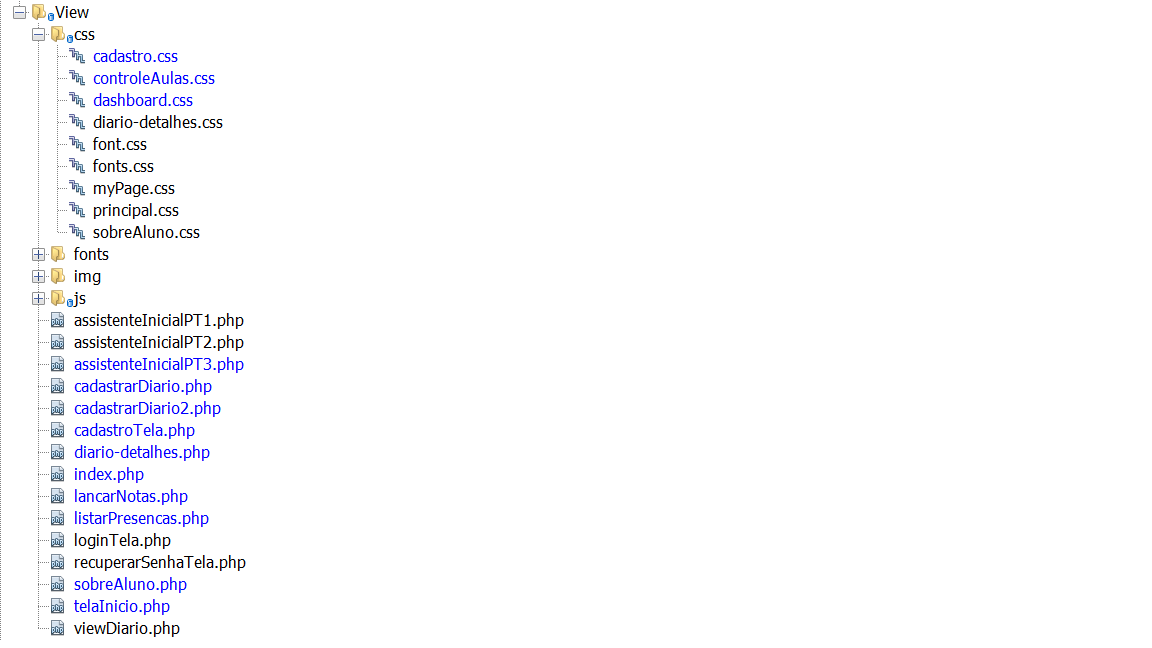
\includegraphics[scale=0.9]{view}\\  % o 0.9 
	\caption{Divisão dos diretórios - view} %legenda
	{\small } %Fonte da imagem
	\label{fig:view} %rotulo para refencia
\end{figure}

No \textit{Model}, estão os objetos e seus respectivos \textit{gets} e \textit{sets}, bem como as classes que estabelecem conexão ao banco de dados e as classes de acesso a dados (DAO - \textit{Date Acess Object}). Essa estruturação permite que quando ocorra mudança nos dados de qualquer objeto, seja fácil a notificação para classes que exercem controle sobre esses dados e o repasse para as classes responsáveis às "visões" do usuários.

A interface se localiza no \textit{View}. Ali estão todos os códigos em HTML, CSS e JS responsáveis pela renderização do conteúdo que interage com o usuário, imagens e fontes tipográficas. Por último, mas não menos importante, temos o diretório \textit{Controller}, onde ficam as principais tarefas e requisições, controladas por comandos em PHP. Em exemplo: toda ação de cadastro de um "professor" é captada por um campo na interface \textit{view} e transmitido para o \textit{controller} "professorInterface.php" que é responsavel por analisar os comandos e direcinar o caminho de cada tipo de ação para sua tarefa, esperar uma resposta e executar uma ação de retorno com essa resposta para a \textit{view}.

Ao entrar no sistema, o usuário se depara com duas opções: se cadastrar ou \textit{logar} no sistema. Na primeira, o usuário insere dados de \textit{e-mail}, senha, nome e imagem de perfil(opcional). Após prosseguir, na \textit{view} os dados são encaminhados para interfaceProfessor.php que chama o \textit{bean} responsável por registrar os dados. Esses dados são devolvidos a ele, que solicita a classe DAO (\textit{Data Access Object}) que armazene os dados no banco. As Figuras \ref{fig:loginoucadastro}, \ref{fig:cadastroview},
 \ref{fig:cadastroview1},
 \ref{fig:cadastroview2},
 \ref{fig:cadastroview3},
 \ref{fig:cadastroview4}, e
 \ref{fig:cadastroview5} respectivamente, mostram os arquivos com o fluxo de dados descrito.
 


\begin{figure}[!htb]
	\centering
	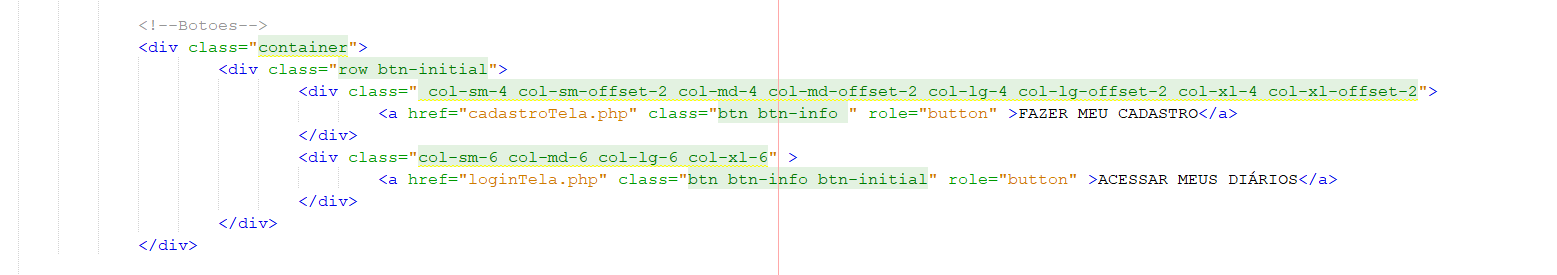
\includegraphics[width=0.9\linewidth]{loginOuCadastro}
	\caption{Arquivo "index.php"}
	\label{fig:loginoucadastro}
\end{figure}

\begin{figure}[!htb]
	\centering
	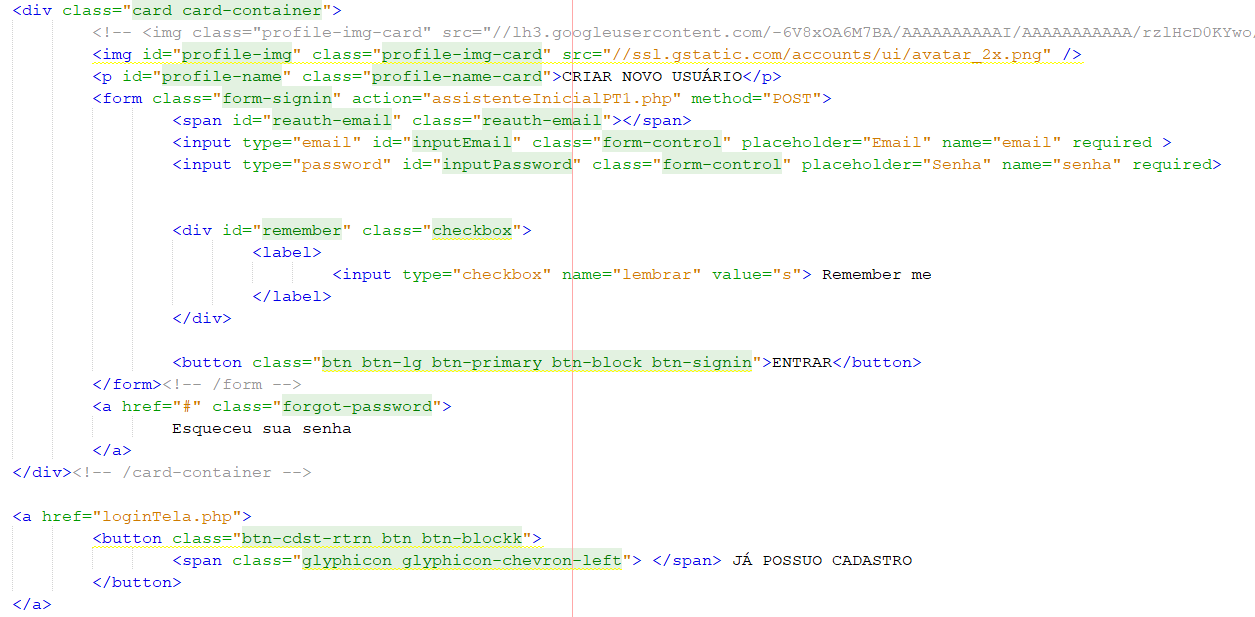
\includegraphics[width=0.9\linewidth]{cadastroView}
	\caption{Arquivo "cadastroTela.php" }
	\label{fig:cadastroview}
\end{figure}

\begin{figure}[!htb]
	\centering
	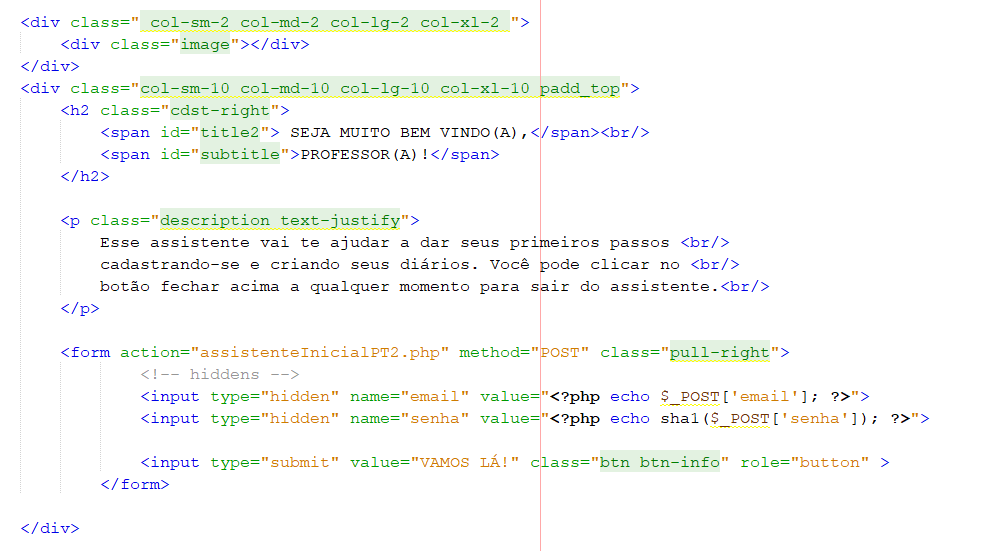
\includegraphics[width=0.9\linewidth]{cadastroView1}
	\caption{Arquivo "assistenteInicialPT1.php"}
	\label{fig:cadastroview1}
\end{figure}


\begin{figure}[!htb]
	\centering
	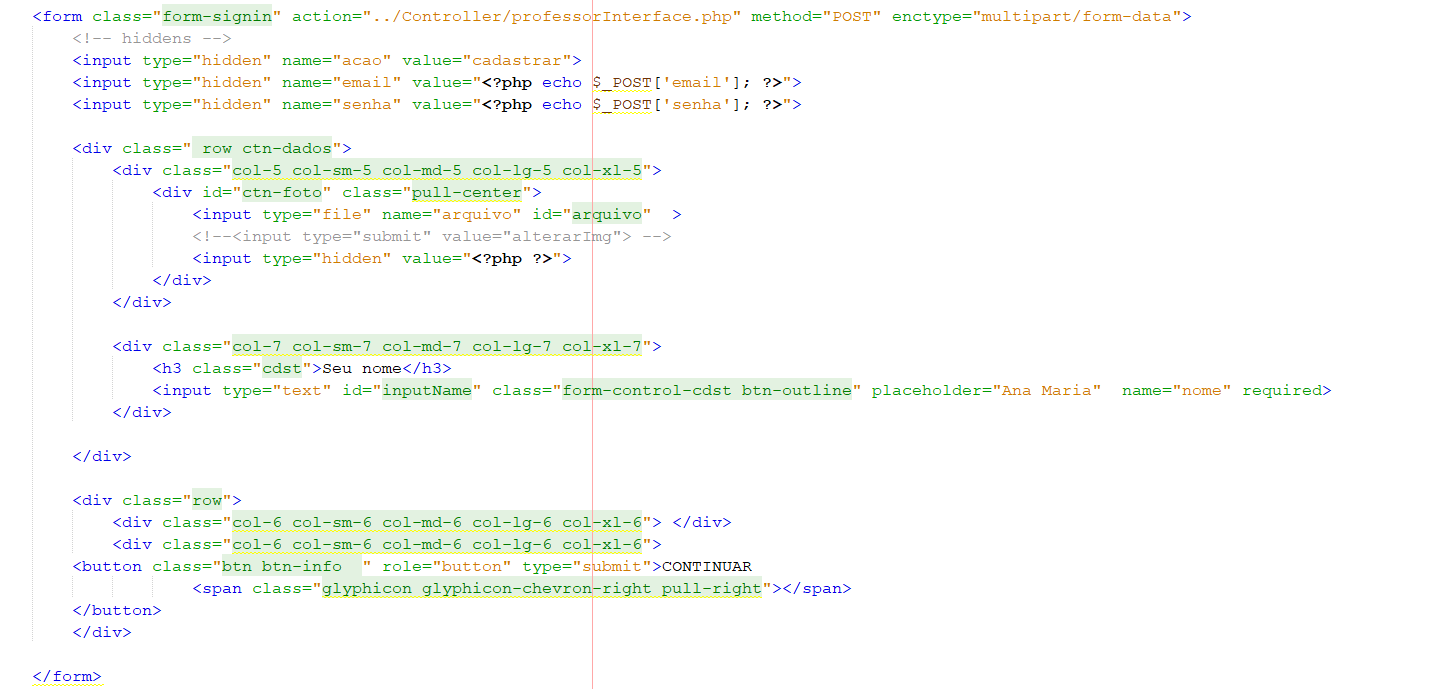
\includegraphics[width=0.9\linewidth]{cadastroView2}
	\caption{Arquivo "assistenteInicialPT2.php"}
	\label{fig:cadastroview2}
\end{figure}

\begin{figure}[!htb]
	\centering
	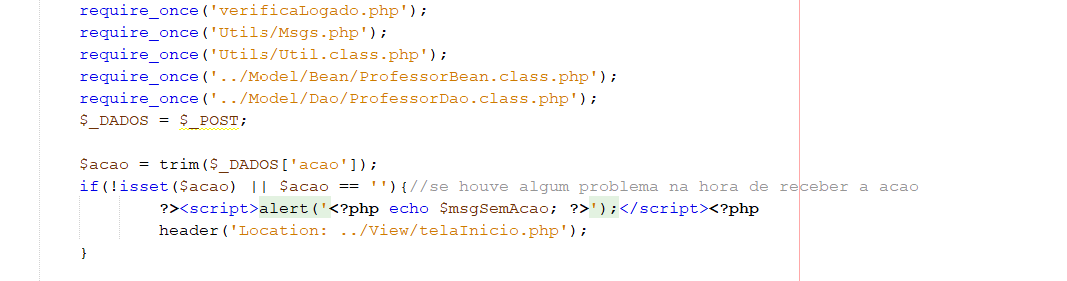
\includegraphics[width=0.9\linewidth]{cadastroView3}
	\caption{Arquivo "assistenteInicialPT3.php"}
	\label{fig:cadastroview3}
\end{figure}

\begin{figure}[!htb]
	\centering
	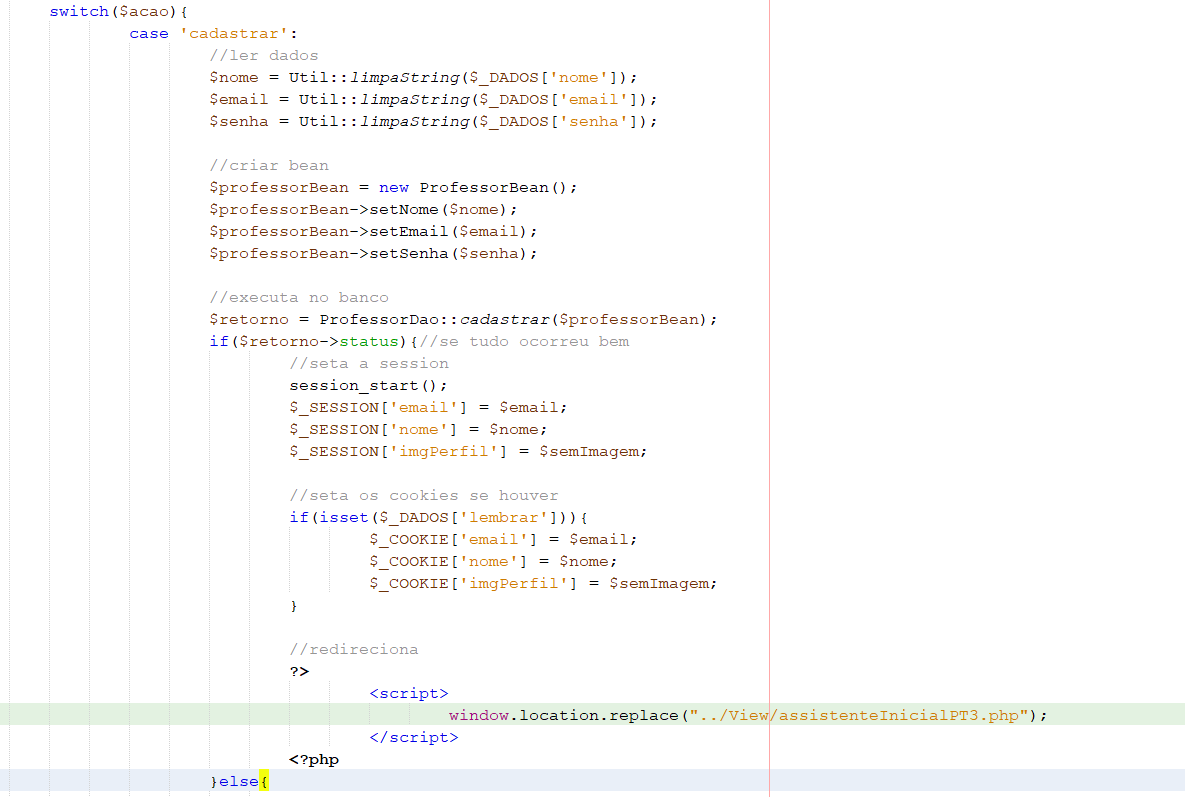
\includegraphics[width=0.9\linewidth]{cadastroView4}
	\caption{Arquivo "professorInterface.php"}
	\label{fig:cadastroview4}
\end{figure}

\begin{figure}[!htb]
	\centering
	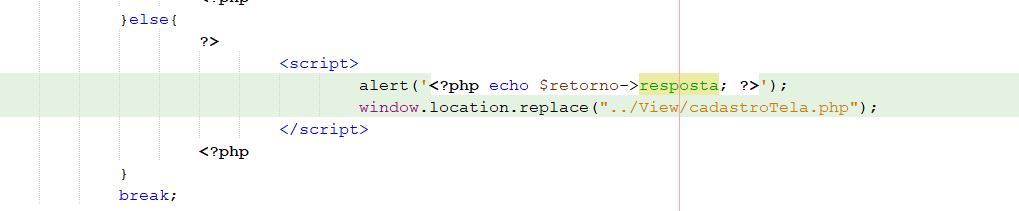
\includegraphics[width=0.9\linewidth]{cadastroView5}
	\caption{Arquivo "professorInterface.php"  - continuação da figura \ref{fig:cadastroview4}}
	\label{fig:cadastroview5}
\end{figure}

As estrutura das classes utilizadas no cadastro acima exemplificado, são mostradas nas figuras \ref{fig:cadastroview6} e \ref{fig:cadastroview7}.

\begin{figure}
	\centering
	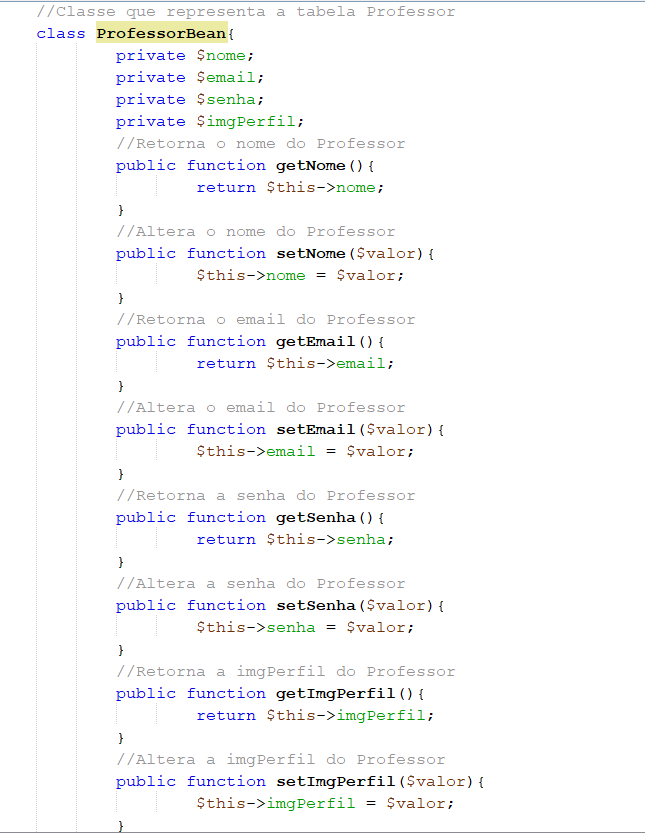
\includegraphics[width=0.9\linewidth]{cadastroView6}
	\caption{Classe "ProfessorBean.class.php"}
	\label{fig:cadastroview6}
\end{figure}

\begin{figure}
	\centering
	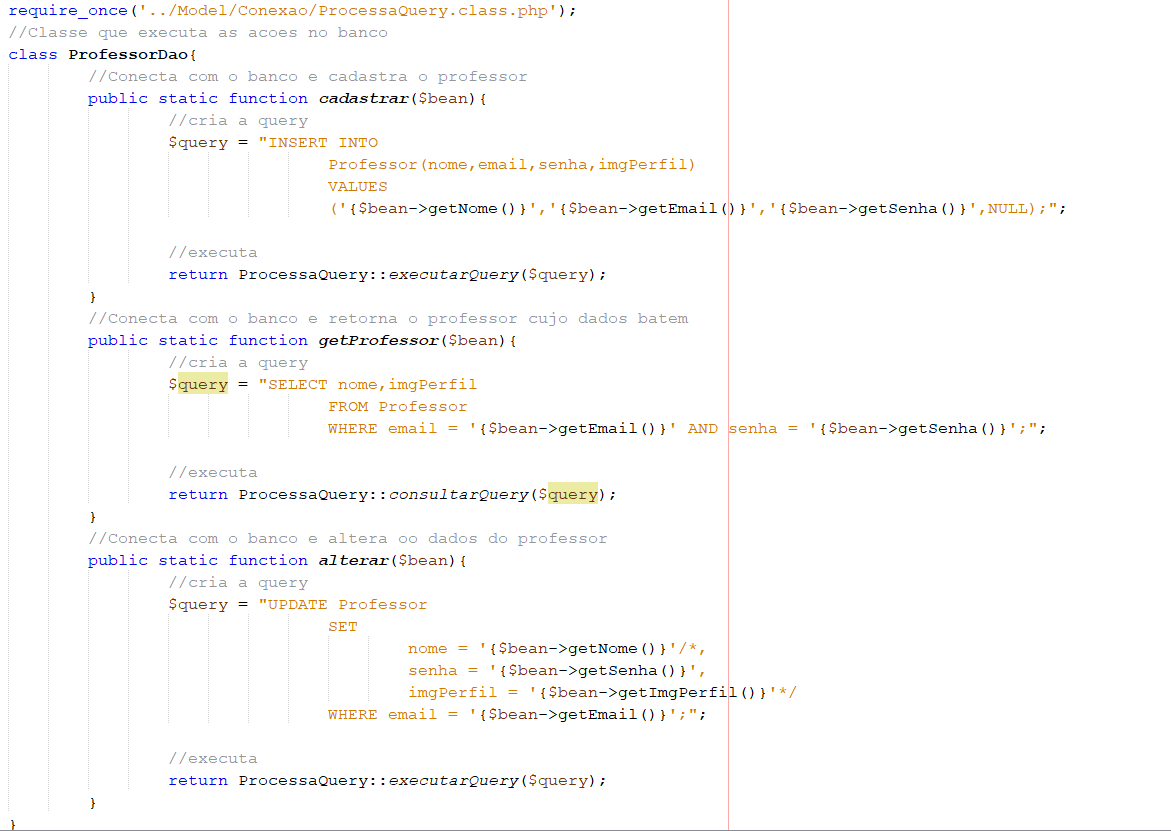
\includegraphics[width=0.9\linewidth]{cadastroView7}
	\caption{Classe "ProfessorDao.php"}
	\label{fig:cadastroview7}
\end{figure}




\section{Testes}

Os testes feitos na aplicação, são baseados no conceito de "teste de caixa branca". Tal tipo de teste (também chamado de estrutural ou verificação) tem por objetivo avaliar a lógica e o comportamento interno de cada componente, avaliando diretamente o código fonte.

Os testes foram feitos durante a fase de desenvolvimento para testar fluxo de dados, inspecionar condições, variáveis e outros, através da utilização da interface gráfica para verificação.


\chapter{RESULTADOS E DISCUSSÃO}
\label{cap:resultados}

\section{Módulo Professor}


O módulo implementado foi o do Professor. Para utilizar os componentes (Aluno, Aula, Avaliação e Diário), o sistema exige autenticação do usuário (Figura \ref{fig:loginTela}). Caso ainda não possua \textit{login}, basta optar pela criação de um novo usuário como mostrado na Figura \ref{fig:index}. O cadastro de professor é uma funcionalidade do módulo e é demonstrado nas Figuras \ref{fig:cadastroTela}, \ref{fig:assistenteInicialPT1}, \ref{fig:assistenteInicialPT2} e \ref{fig:assistenteInicialPT3}. Após terminar seu cadastro pessoal, o professor cria seu primeiro diário, que será demostrado posteriormente. Todas figuras aqui apresentadas, simulam o cadastro do professor fictício nomeado "Mallú Eduarda".

Finalizando esse processo, a página inicial é demostrada na Figura \ref{fig:telaInicio}. 

% Tela inicial da aplicação
\begin{figure}[!htb]
	\centering
	\caption{Tela inicial da aplicação} %legenda
	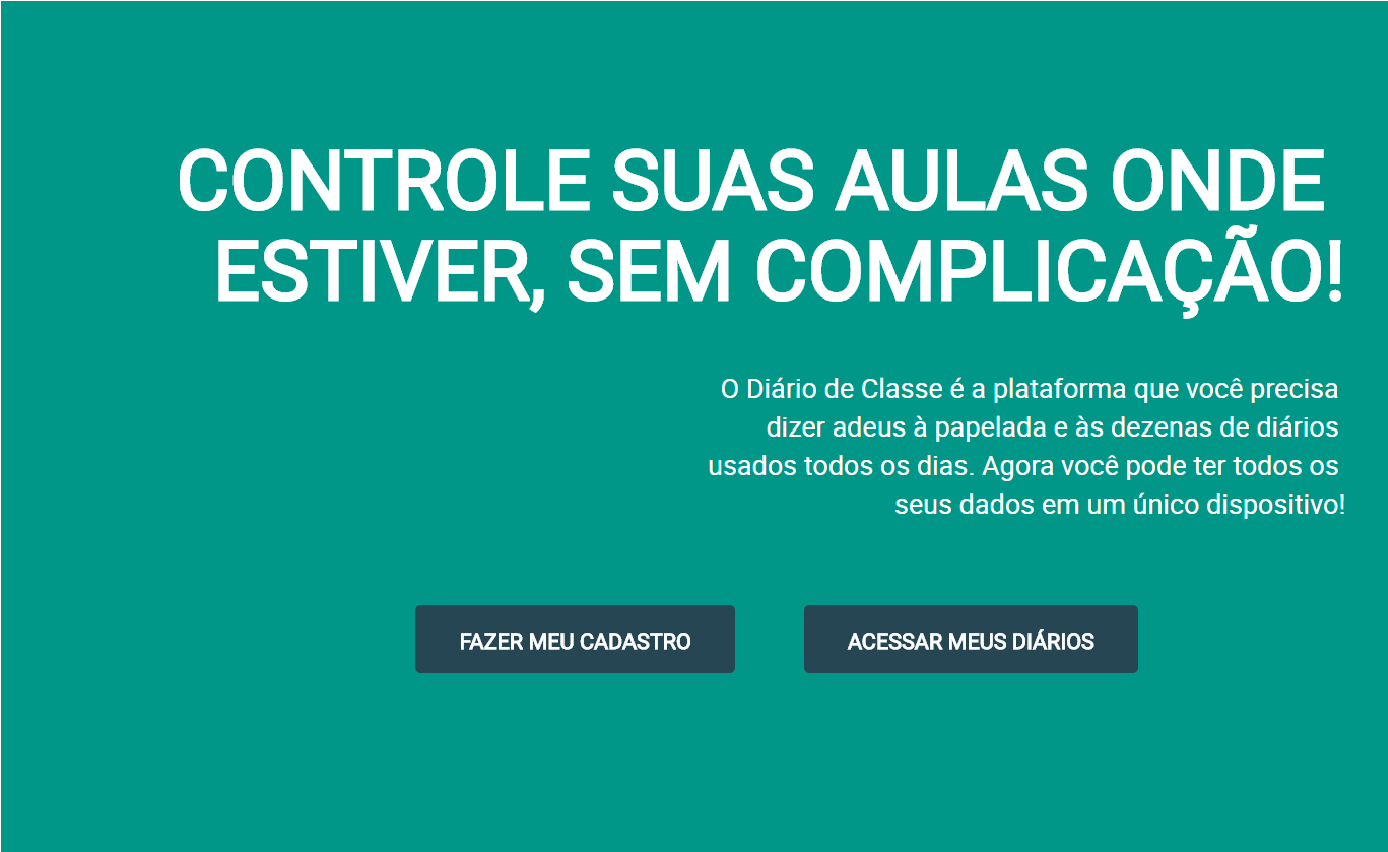
\includegraphics[scale=0.4]{index}\\  % o 0.9 indica 90% do tamanho original
	% pdfLaTeX aceita figuras no formato PNG, JPG ou PDF
	% figuras vetoriais podem ser exportadas para eps e depois convertidas para pdf usando epstopdf
	{\small } %Fonte da imagem
	\label{fig:index} %rotulo para refencia
\end{figure}

% Tela de cadastro
\begin{figure}[!htb]
	\centering
	\caption{Tela de cadastro de usuário} %legenda
	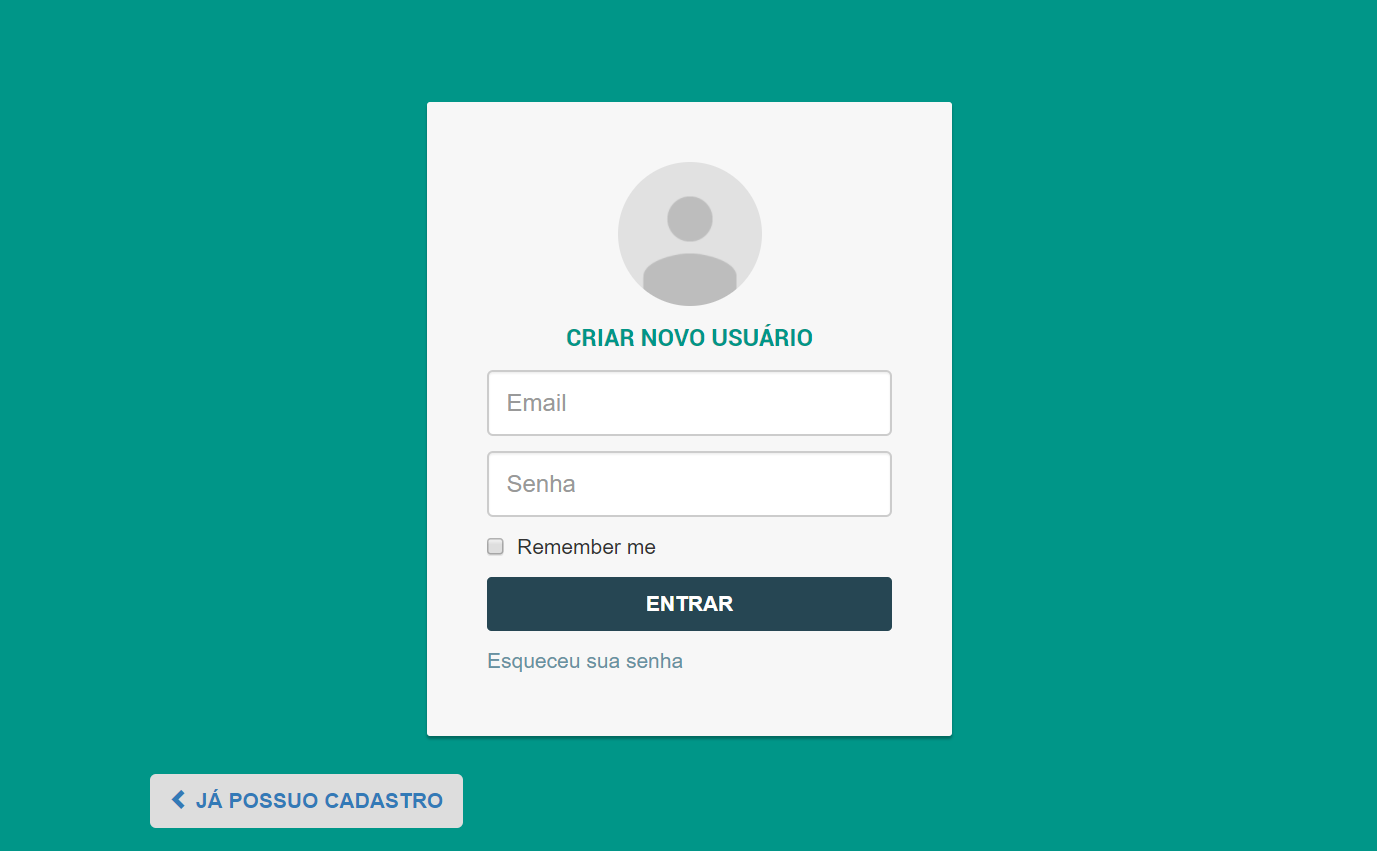
\includegraphics[scale=0.4]{cadastroTela}\\  % o 0.9 indica 90% do tamanho original
	% pdfLaTeX aceita figuras no formato PNG, JPG ou PDF
	% figuras vetoriais podem ser exportadas para eps e depois convertidas para pdf usando epstopdf
	{\small } %Fonte da imagem
	\label{fig:cadastroTela} %rotulo para refencia
\end{figure}


% Assistente Inicial pt1
\begin{figure}[!htb]
	\centering
	\caption{Assistente inicial: parte 1} %legenda
	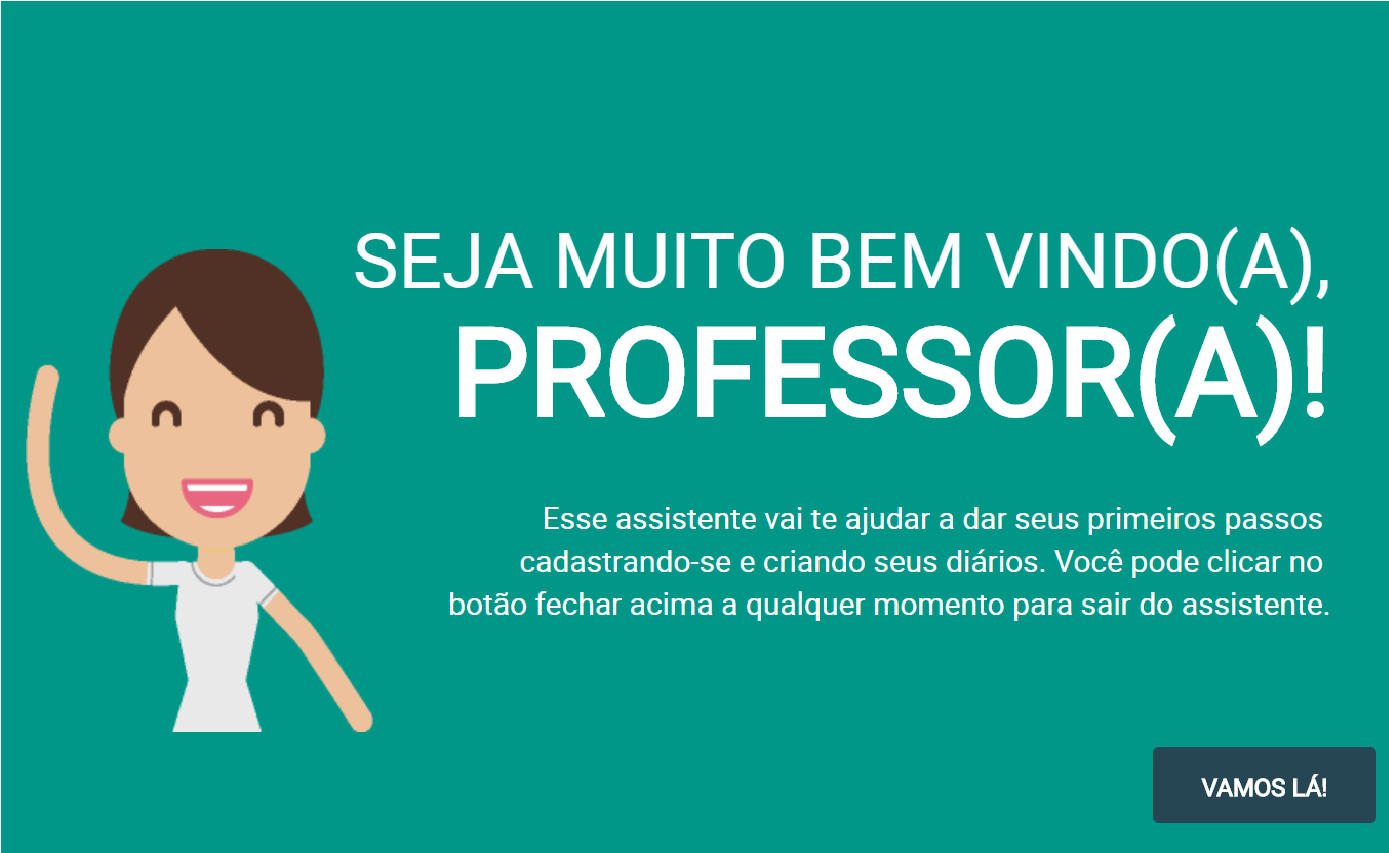
\includegraphics[scale=0.4]{assistenteInicialPT1}\\  % o 0.9 indica 90% do tamanho original
	% pdfLaTeX aceita figuras no formato PNG, JPG ou PDF
	% figuras vetoriais podem ser exportadas para eps e depois convertidas para pdf usando epstopdf
	{\small } %Fonte da imagem
	\label{fig:assistenteInicialPT1} %rotulo para refencia
\end{figure}

% Assistente Inicial pt2
\begin{figure}[!htb]
	\centering
	\caption{Assistente inicial: parte 2} %legenda
	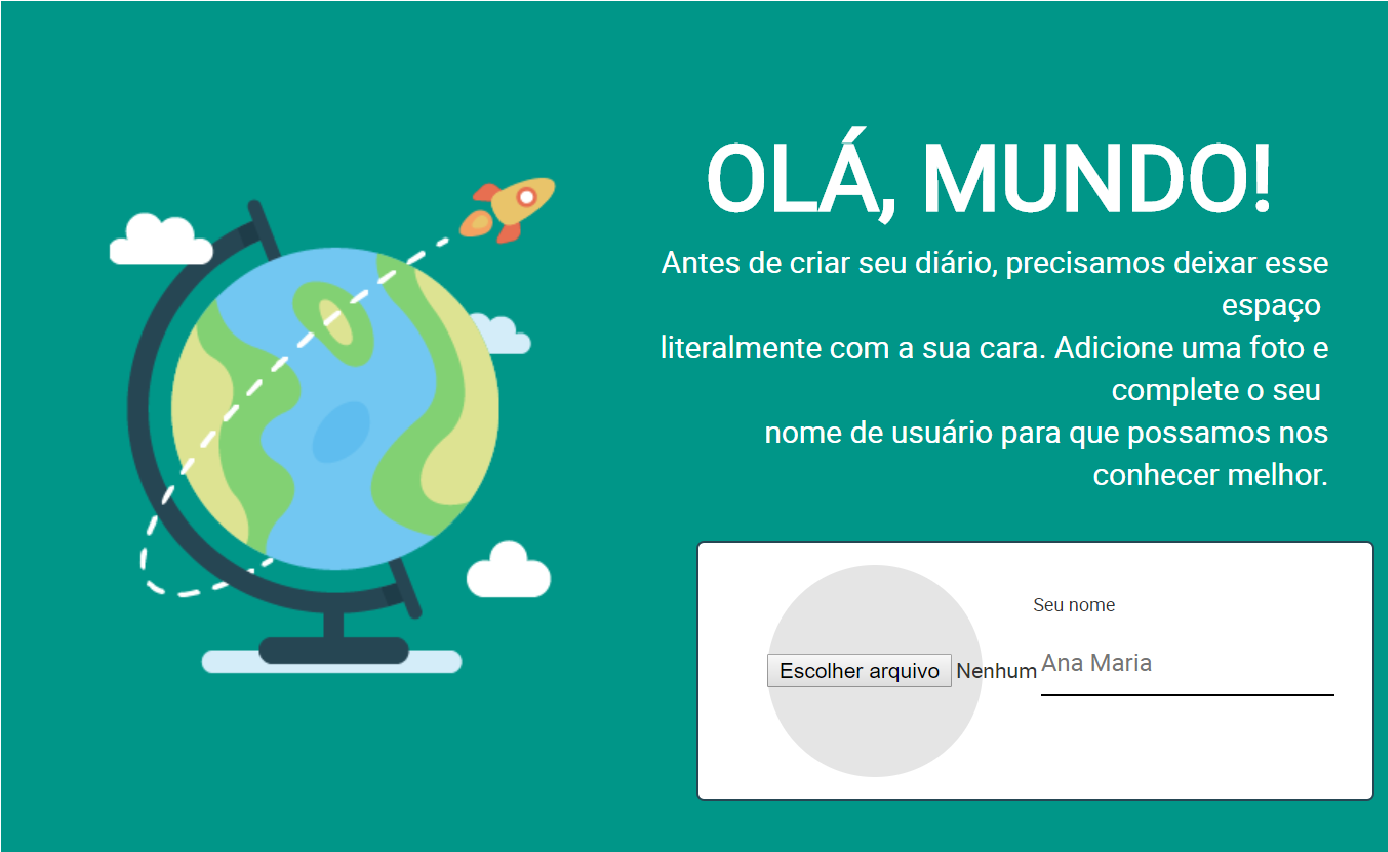
\includegraphics[scale=0.4]{assistenteInicialPT2}\\  % o 0.9 indica 90% do tamanho original
	% pdfLaTeX aceita figuras no formato PNG, JPG ou PDF
	% figuras vetoriais podem ser exportadas para eps e depois convertidas para pdf usando epstopdf
	{\small } %Fonte da imagem
	\label{fig:assistenteInicialPT2} %rotulo para refencia
\end{figure}

% Assistente Inicial pt3
\begin{figure}[!htb]
	\centering
	\caption{Assistente inicial: parte 3} %legenda
	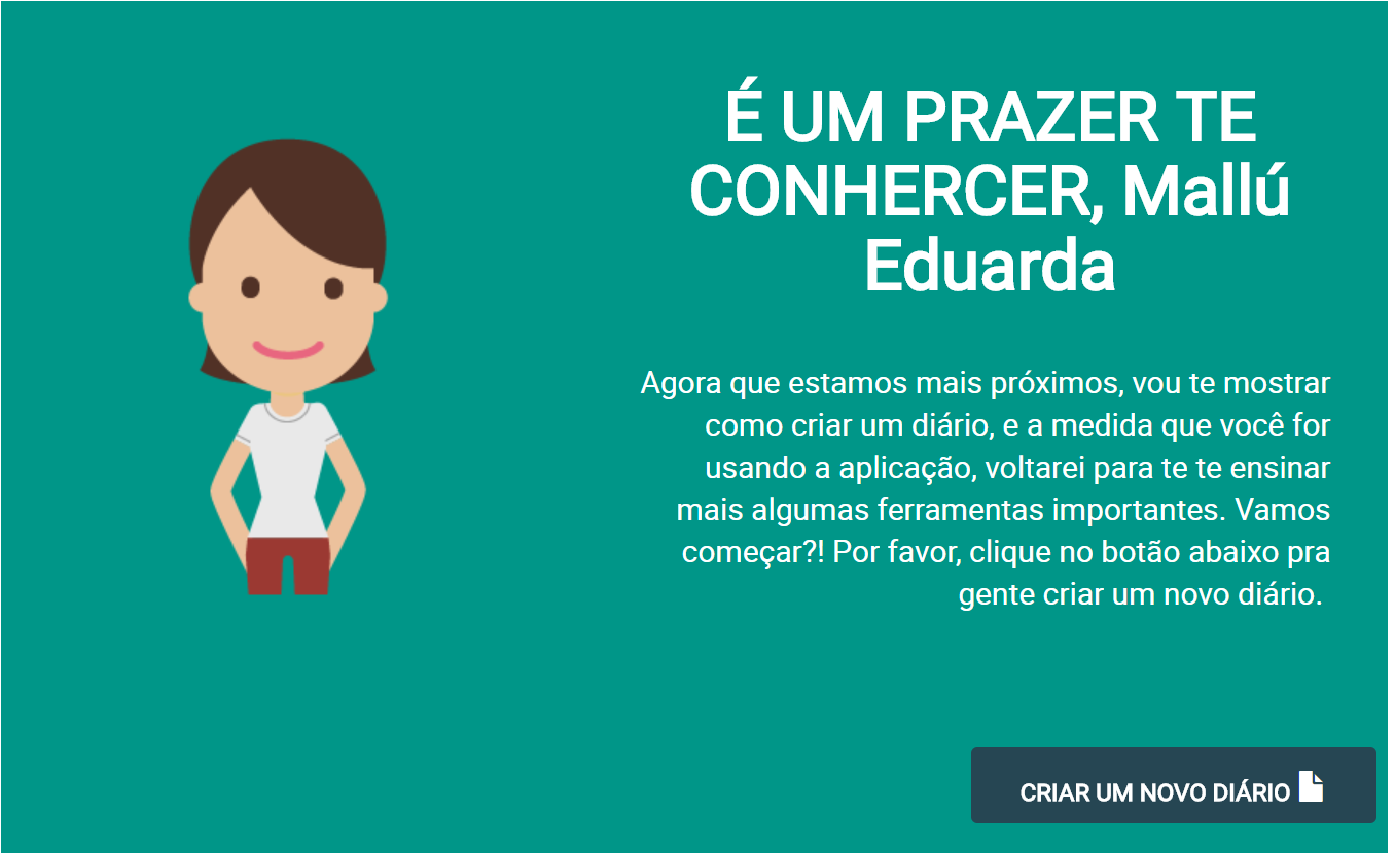
\includegraphics[scale=0.4]{assistenteInicialPT3}\\  % o 0.9 indica 90% do tamanho original
	% pdfLaTeX aceita figuras no formato PNG, JPG ou PDF
	% figuras vetoriais podem ser exportadas para eps e depois convertidas para pdf usando epstopdf
	{\small } %Fonte da imagem
	\label{fig:assistenteInicialPT3} %rotulo para refencia
\end{figure}

%Tela de login
\begin{figure}[!htb]
	\centering
	\caption{Tela de login} %legenda
	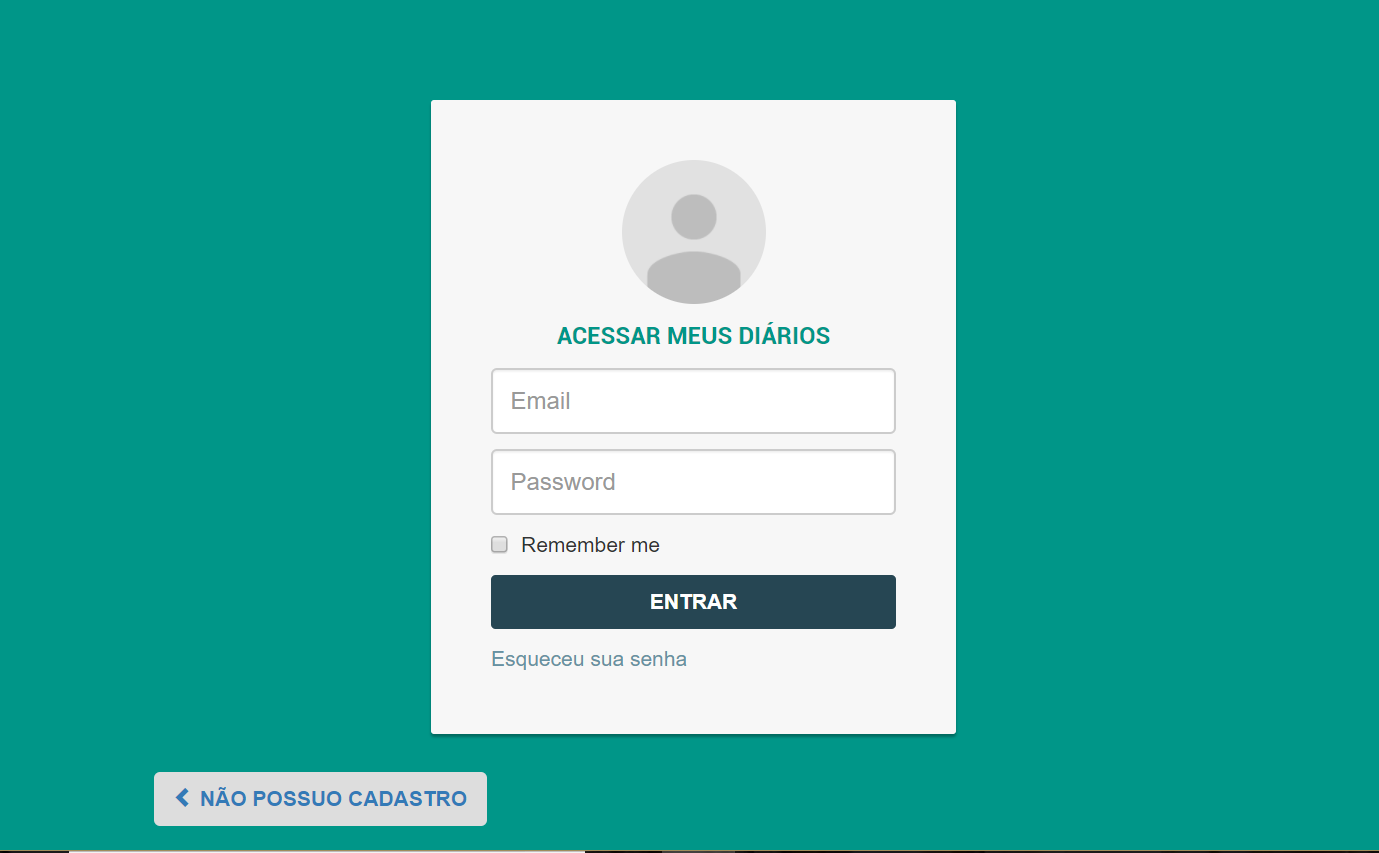
\includegraphics[scale=0.4]{loginTela}\\  % o 0.9 indica 90% do tamanho original
	% pdfLaTeX aceita figuras no formato PNG, JPG ou PDF
	% figuras vetoriais podem ser exportadas para eps e depois convertidas para pdf usando epstopdf
	{\small } %Fonte da imagem
	\label{fig:loginTela} %rotulo para refencia
\end{figure}

%pagina inicial professor
\begin{figure}[!htb]
	\centering
	\caption{Pagina inicial do professor} %legenda
	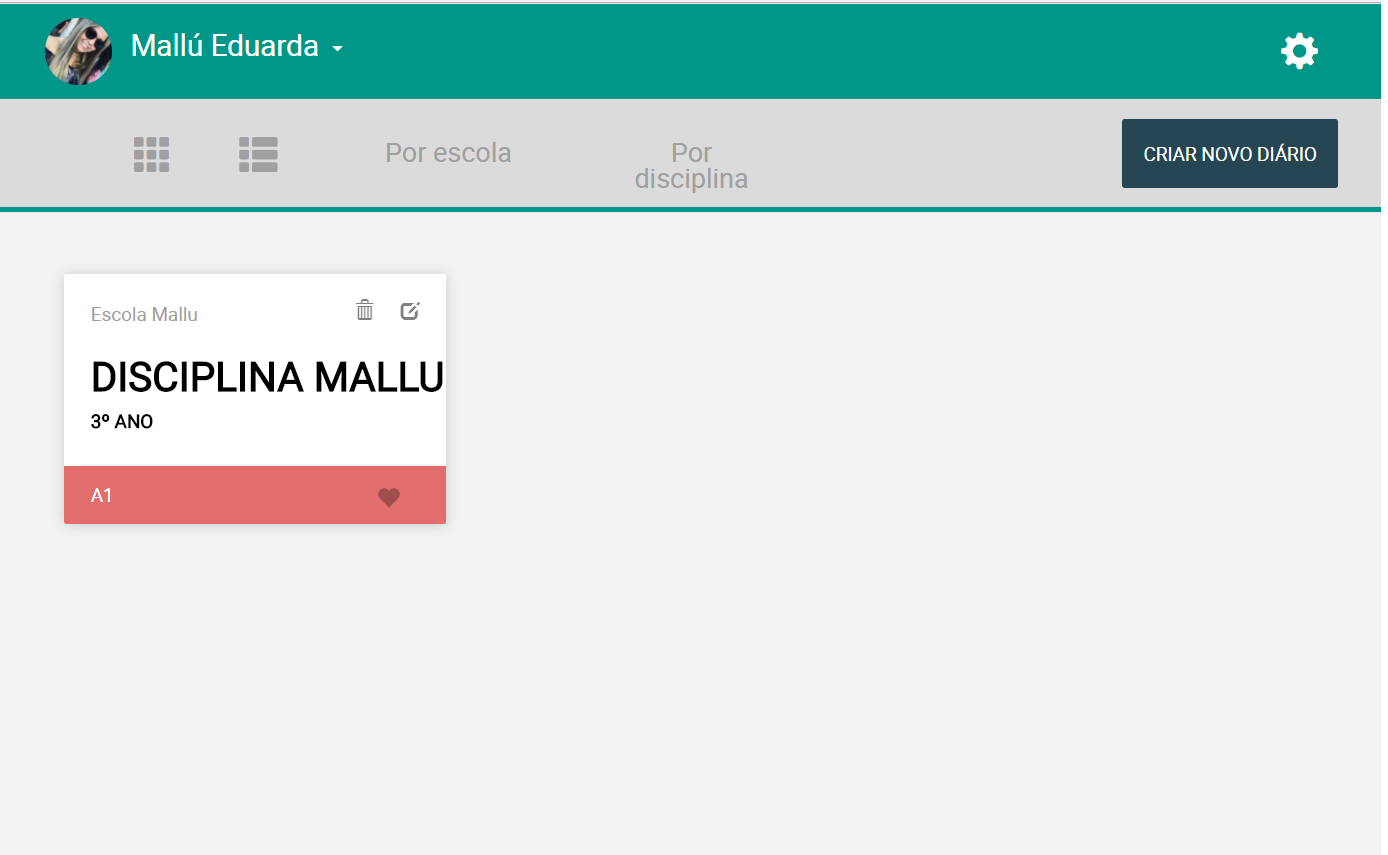
\includegraphics[scale=0.4]{telaInicio}\\  % o 0.9 indica 90% do tamanho original
	% pdfLaTeX aceita figuras no formato PNG, JPG ou PDF
	% figuras vetoriais podem ser exportadas para eps e depois convertidas para pdf usando epstopdf
	{\small } %Fonte da imagem
	\label{fig:telaInicio} %rotulo para refencia
\end{figure}


\section{Componentes}

Aqui são citados e explicados os componentes do sistema.

\subsection{Diário}

Como componente principal, portador de todas as informações relevantes ao registro da prática pedagógica do professor, o diário de classe desempenha papel fundamental e único no módulo. As funcionalidades são: cadastrar, editar, excluir e visualizar diário. As mesmas, serão numeradas e explicadas posteriormente.

A função que carrega as informações e controla as requisições do usuário dentro de cada diário, é mostrada na figura \ref{fig:efetuaAcoes}. Cada clique em uma função é redirecionado para uma ação.


%controlador de ações do diário
\begin{figure}[!htb]
	\centering
	\caption{ Controlador de ações } %legenda
	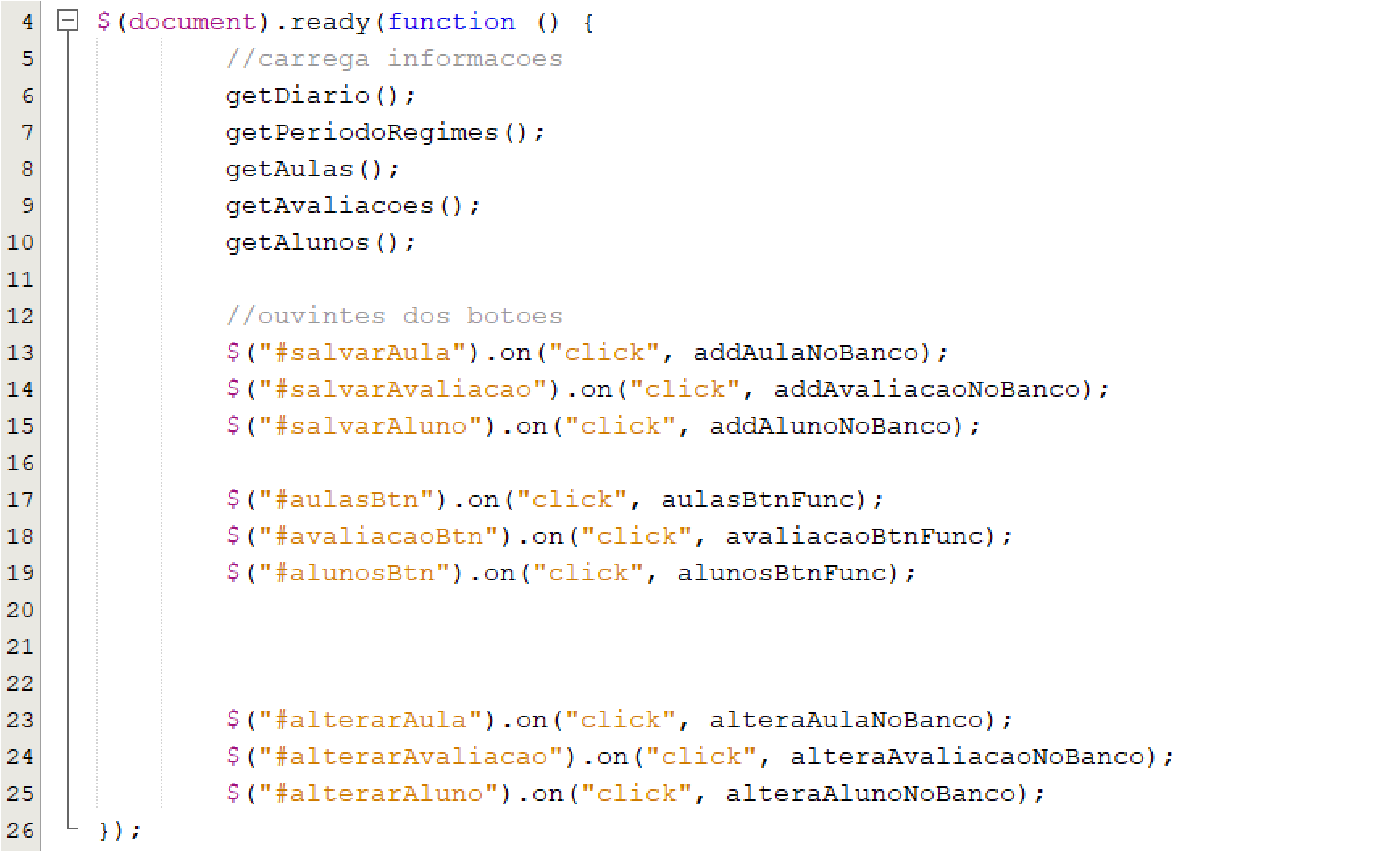
\includegraphics[scale=0.4]{efetuaAcoes}\\  % 
	{\small } %Fonte da imagem
	\label{fig:efetuaAcoes} %rotulo para refencia
\end{figure}


\begin{enumerate}
	\item Cadastrar:
	
	Na tela principal do usuário, existe o botão para cadastro de um novo diário. As informações solicitadas condizem com as presente no diário de papel, que é utilizado pelos professores. São solicitados o nome da escola, nome da disciplina, modalidade, série, identificação da turma e regime de aulas, como mostrado na Figura \ref{fig:cadastrarDiario}. Após a confirmação de preenchimento dos dados, eles são passados para próxima página, para completar o cadastro.
	
	 Nessa segunda parte, são solicitados dados referentes ao regime de aulas, definindo os períodos letivos, datas de início e fim para cada um, quantidade de aulas e o valor (em pontos) estipulado para o mesmo (Figura \ref{fig:cadastrarDiario2}). Essas informações são passadas ao controlador, que capta a "ação" pelo método POST, trata os dados necessários, cria o bean, executa no banco através do dao e redireciona para tela correspondente. Em caso de erro nesse processo, o usuário é informado e redirecionado para recadastrar os dados. Do contrário, a tela inicial com os diários cadastrados é retornada.
	
	
	
	%cadastrarDiario
	\begin{figure}[!htb]
		\centering
		\caption{Cadastrar Diário: parte 1} %legenda
		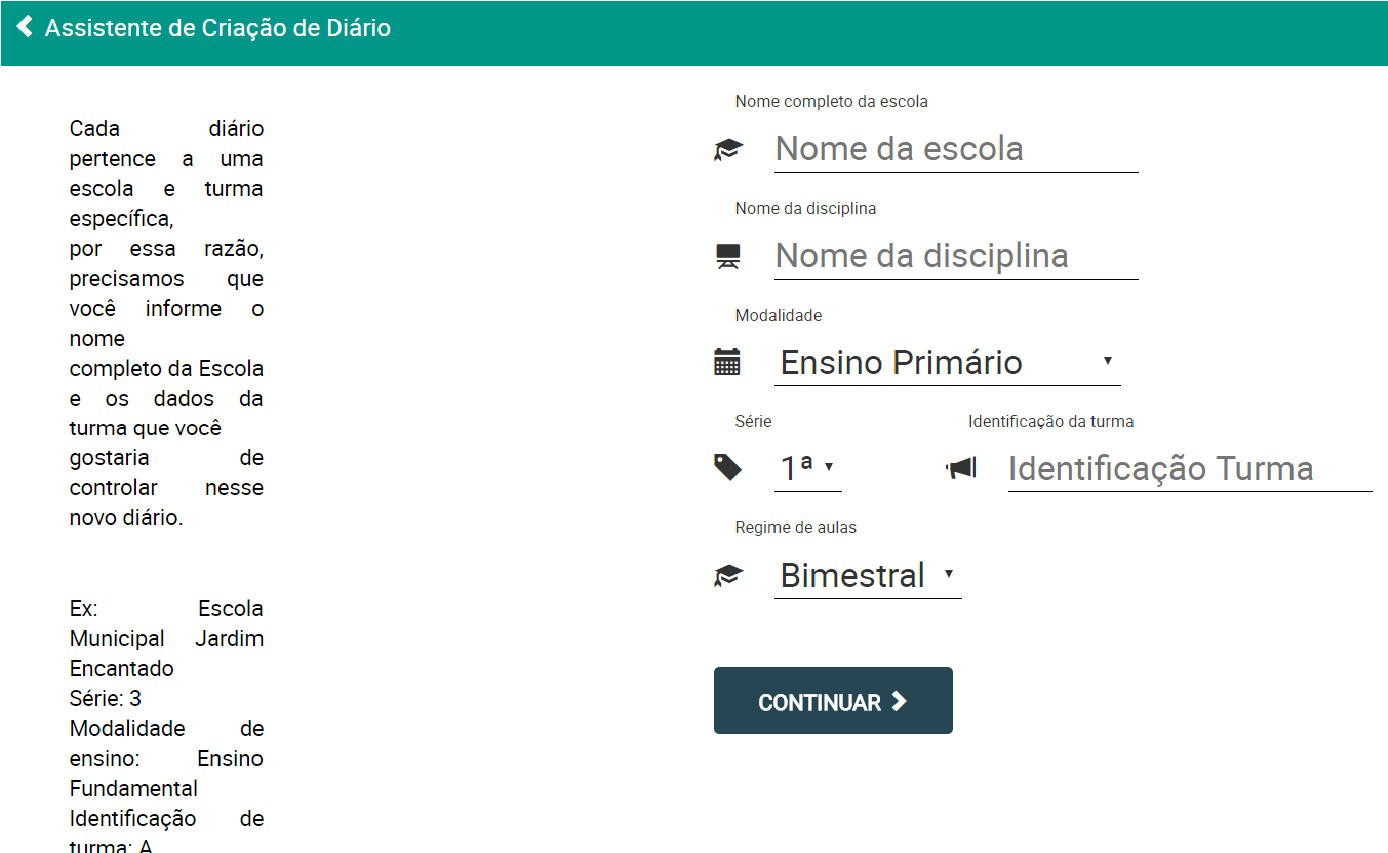
\includegraphics[scale=0.4]{cadastrarDiario}\\  % o 0.9 indica 90% do tamanho 
		{\small } %Fonte da imagem
		\label{fig:cadastrarDiario} %rotulo para refencia
	\end{figure}
	
	%cadastrarDiario2
	\begin{figure}[!htb]
		\centering
		\caption{Cadastrar Diário: parte 2} %legenda
		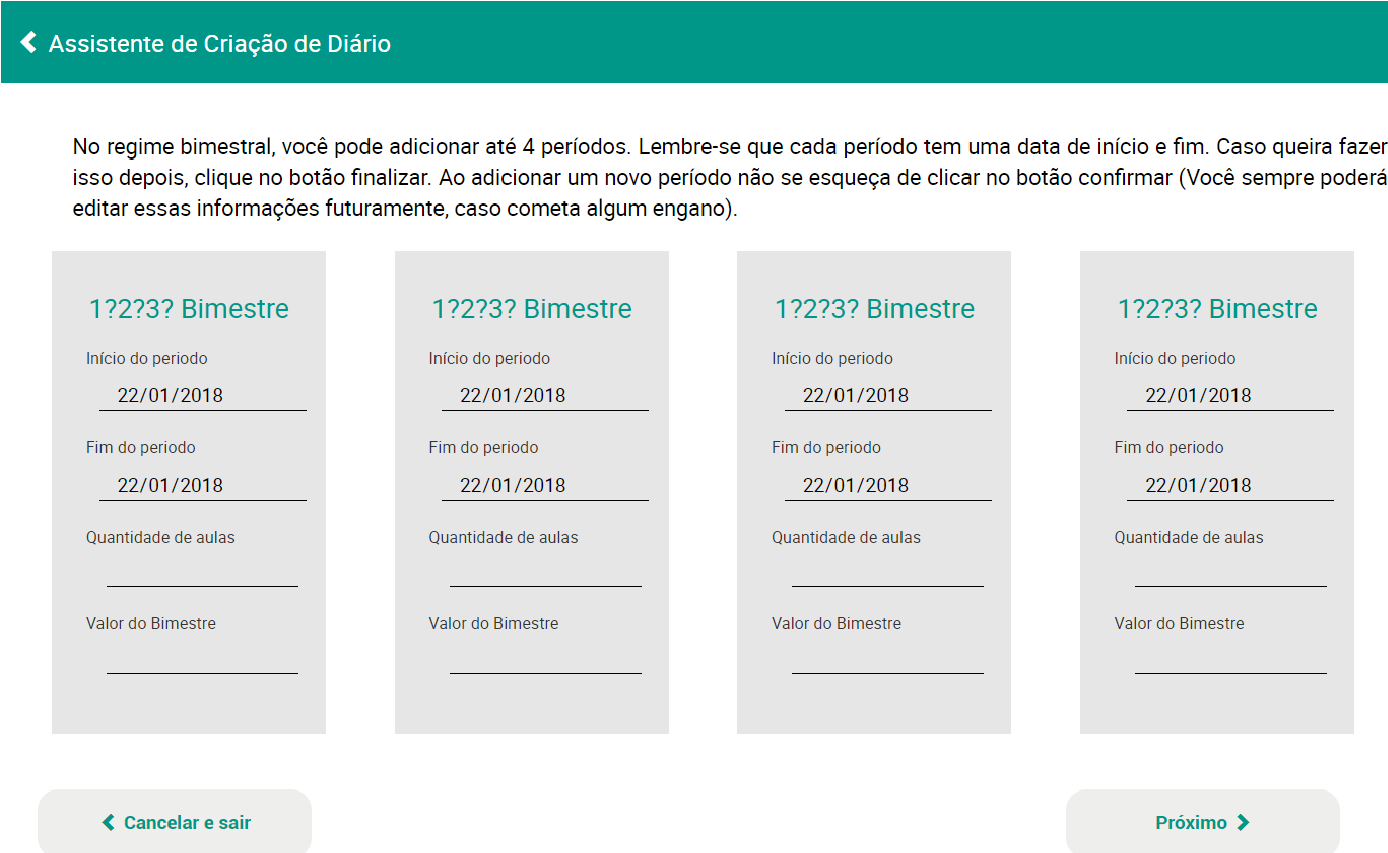
\includegraphics[scale=0.4]{cadastrarDiario2}\\ 
		{\small } %Fonte da imagem
		\label{fig:cadastrarDiario2} %rotulo para refencia
	\end{figure}		
		

	\item Editar:
	
	Ao optar pela edição do conteúdo, os dados são retornados para visão do usuário, advindos do banco de dados (Figuras \ref{fig:editarDiario} e  \ref{fig:editarDiario2}).
	
	%editarDiario
	\begin{figure}[!htb]
		\centering
		\caption{Editar Diário: parte 1} %legenda
		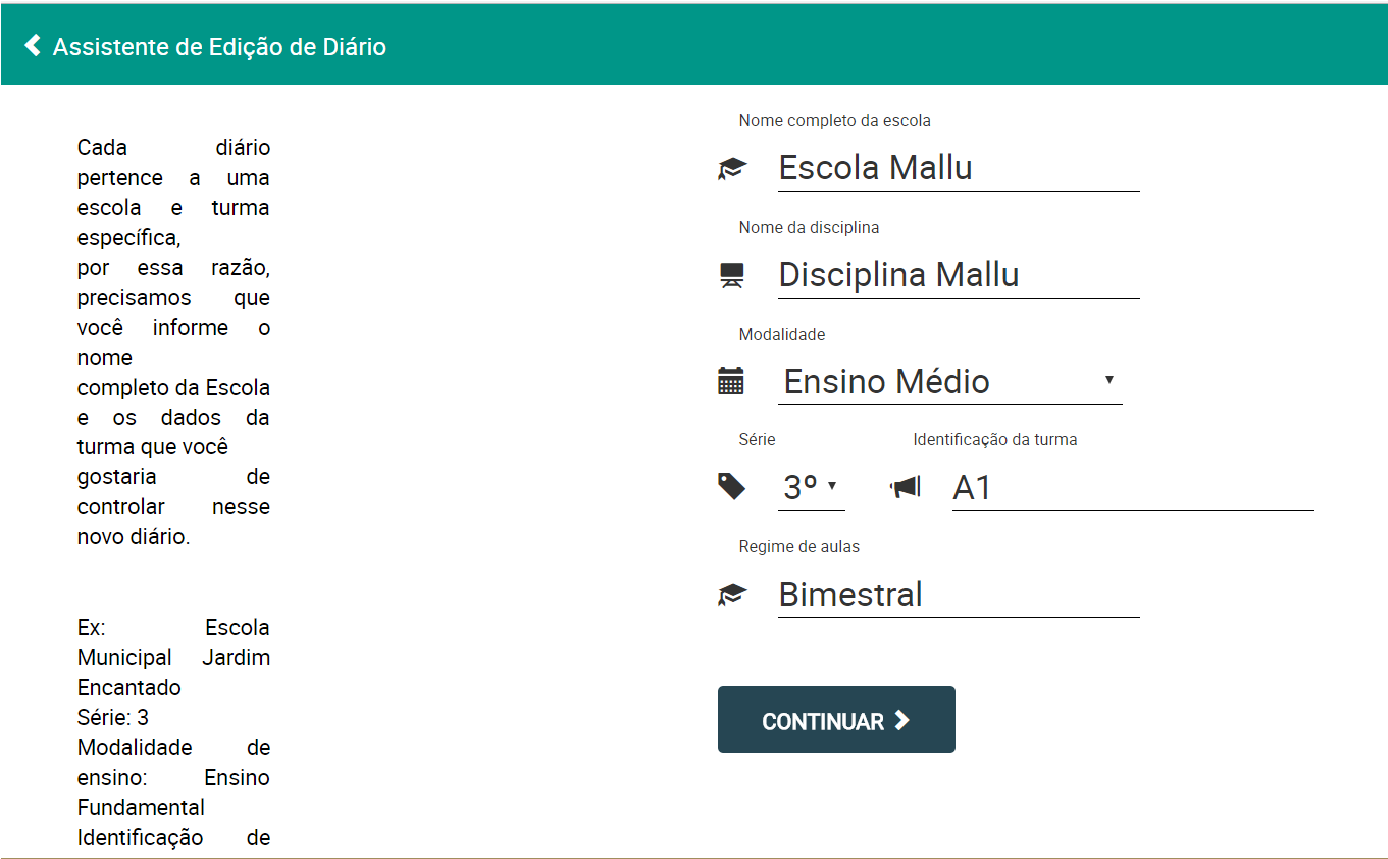
\includegraphics[scale=0.4]{editarDiario}\\  
		{\small } %Fonte da imagem
		\label{fig:editarDiario} %rotulo para refencia
	\end{figure}
	
		%editarDiario2
	\begin{figure}[!htb]
		\centering
		\caption{Editar Diário: parte 2} %legenda
		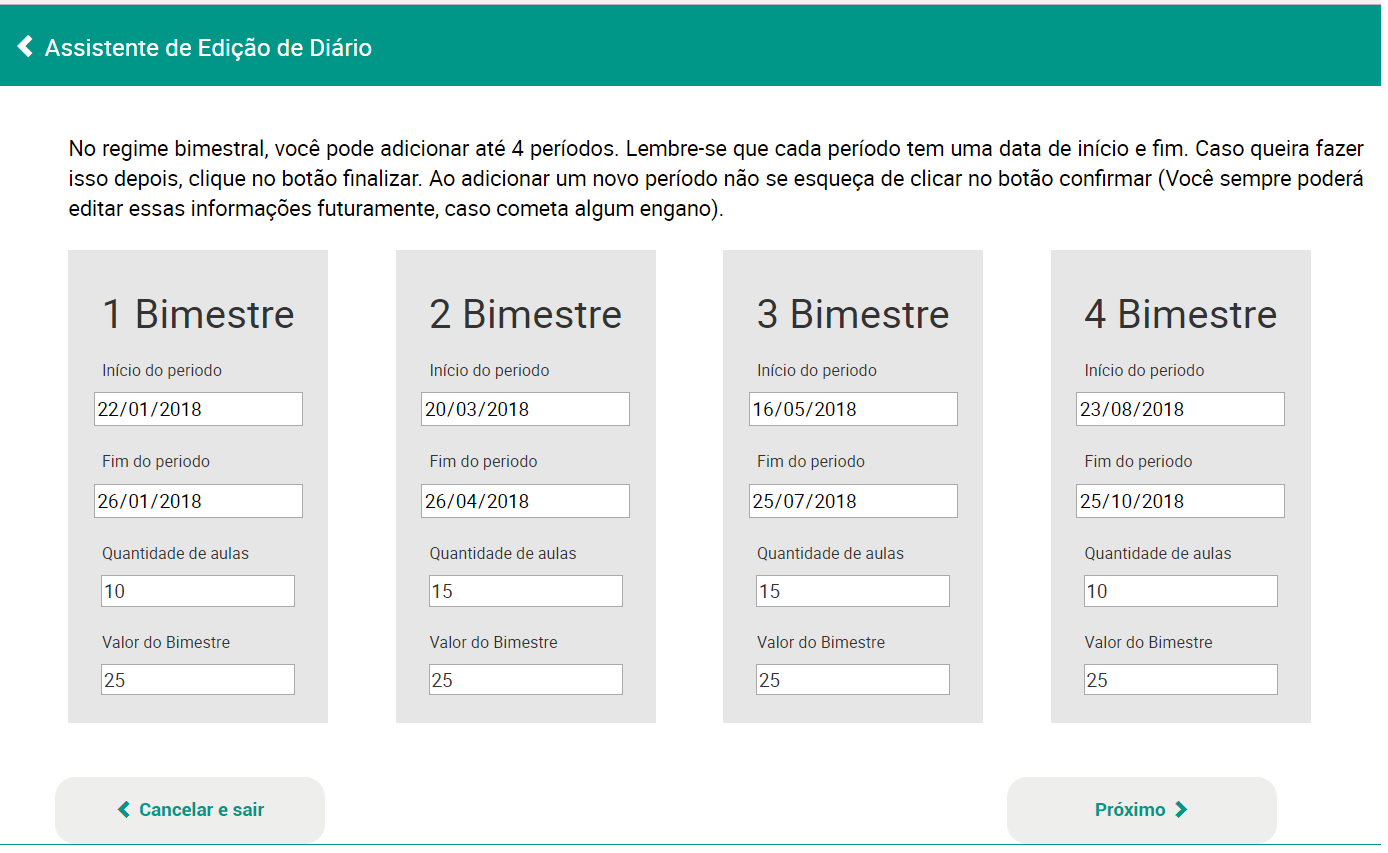
\includegraphics[scale=0.4]{editarDiario2}\\  
		{\small } %Fonte da imagem
		\label{fig:editarDiario2} %rotulo para refencia
	\end{figure}
	
	
	
	
	
	\item Excluir:
	
	Ao excluir um diário, as informações são apagadas da base de dados. 
	
	\item Visualizar:
	
	Os dados são dispostos para o usuário, em forma de acesso aos outros componentes. Pra complementar as informações do diário, podem ser adicionados alunos, aulas e avaliações ao diário. A figura 4.14 mostra o carregamento da pagina inicial do diário.
	
\end{enumerate}



\subsection{Aluno}

Os alunos de uma instituição, realizam seu cadastro por meio da secretaria. Esses dados são repassados diretamente para os professores, pela lista de chamada, através do diário de classe. O mesmo, possui acesso somente ao nome desses alunos.

Entretanto, nesse módulo, essas informações são inseridas manualmente como funcionalidade do sistema, pois não existe outro módulo senão o do professor. É possível cadastrar, editar, excluir, visualizar o boletim de cada aluno e visualizar os alunos.

%cadastrar aluno
\begin{figure}[!htb]
	\centering
	\caption{Cadastro de Aluno} %legenda
	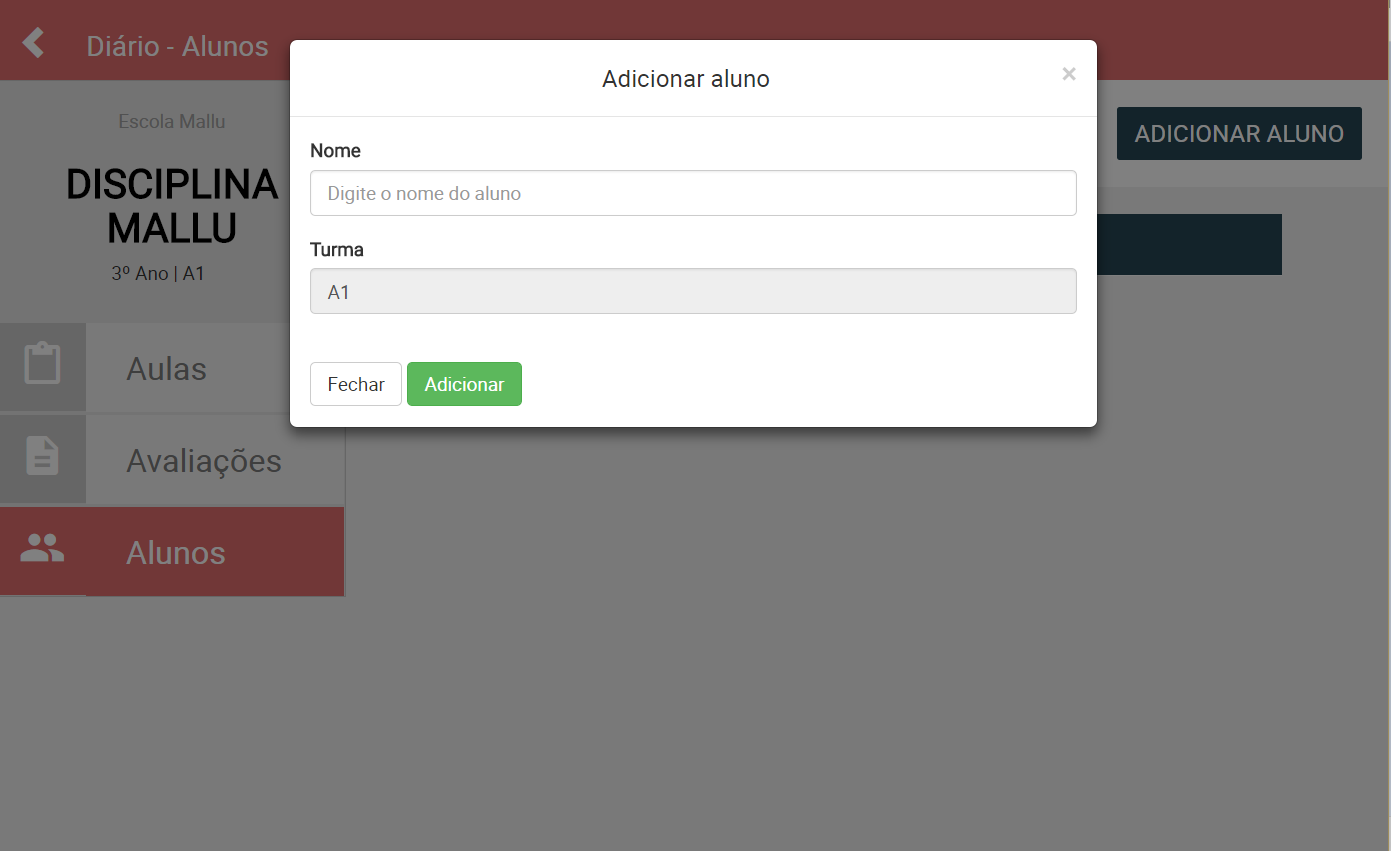
\includegraphics[scale=0.4]{cadastrarAluno}\\  % 
	{\small } %Fonte da imagem
	\label{fig:cadastrarAluno} %rotulo para refencia
\end{figure}

%visualizar aulas
\begin{figure}[!htb]
	\centering
	\caption{Visualização dos Alunos } %legenda
	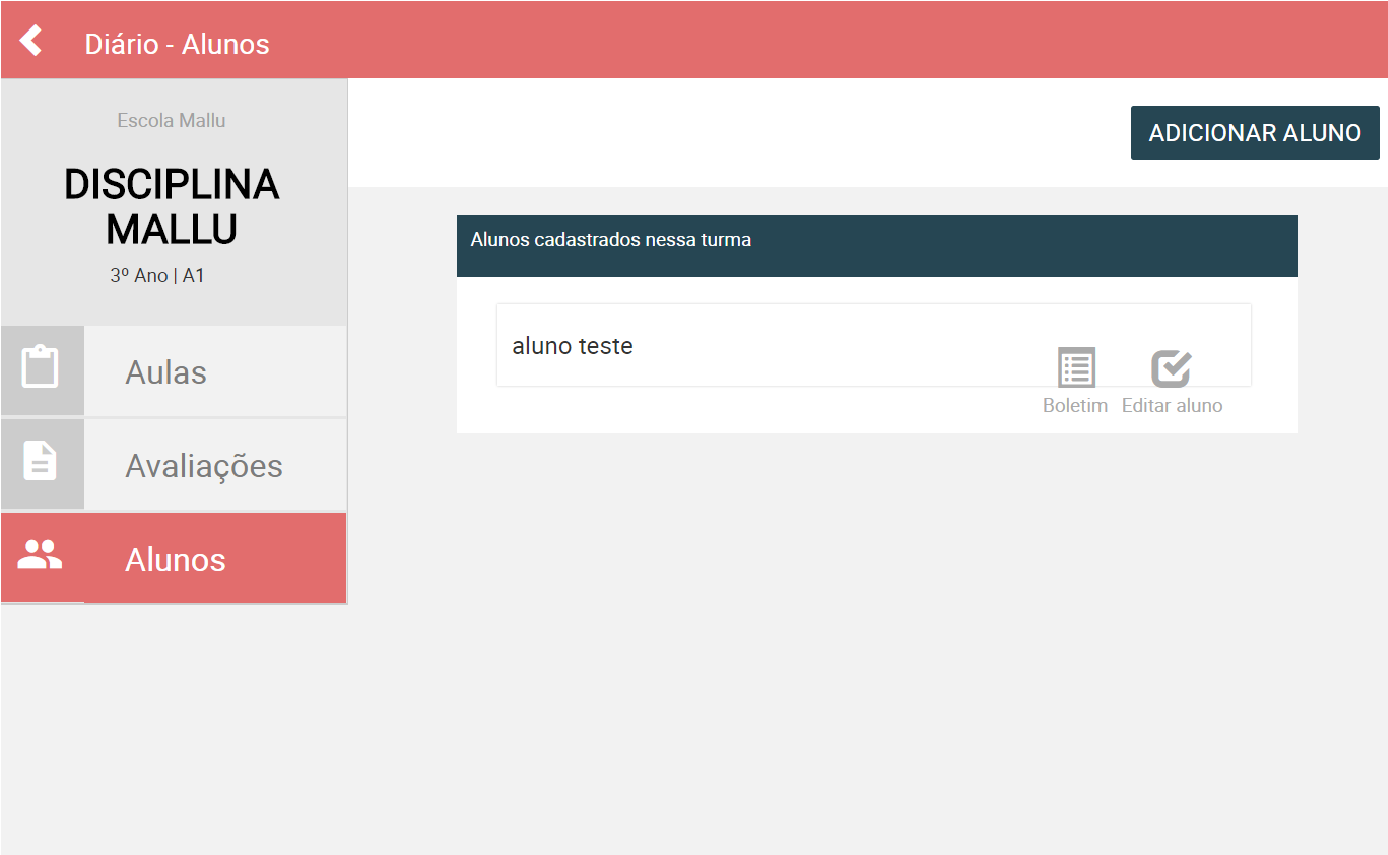
\includegraphics[scale=0.4]{visualizaAlunos}\\  % 
	{\small } %Fonte da imagem
	\label{visualizaAlunos} %rotulo para refencia
\end{figure}

%boletim
\begin{figure}[!htb]
	\centering
	\caption{Visualização do boletim do Aluno } %legenda
	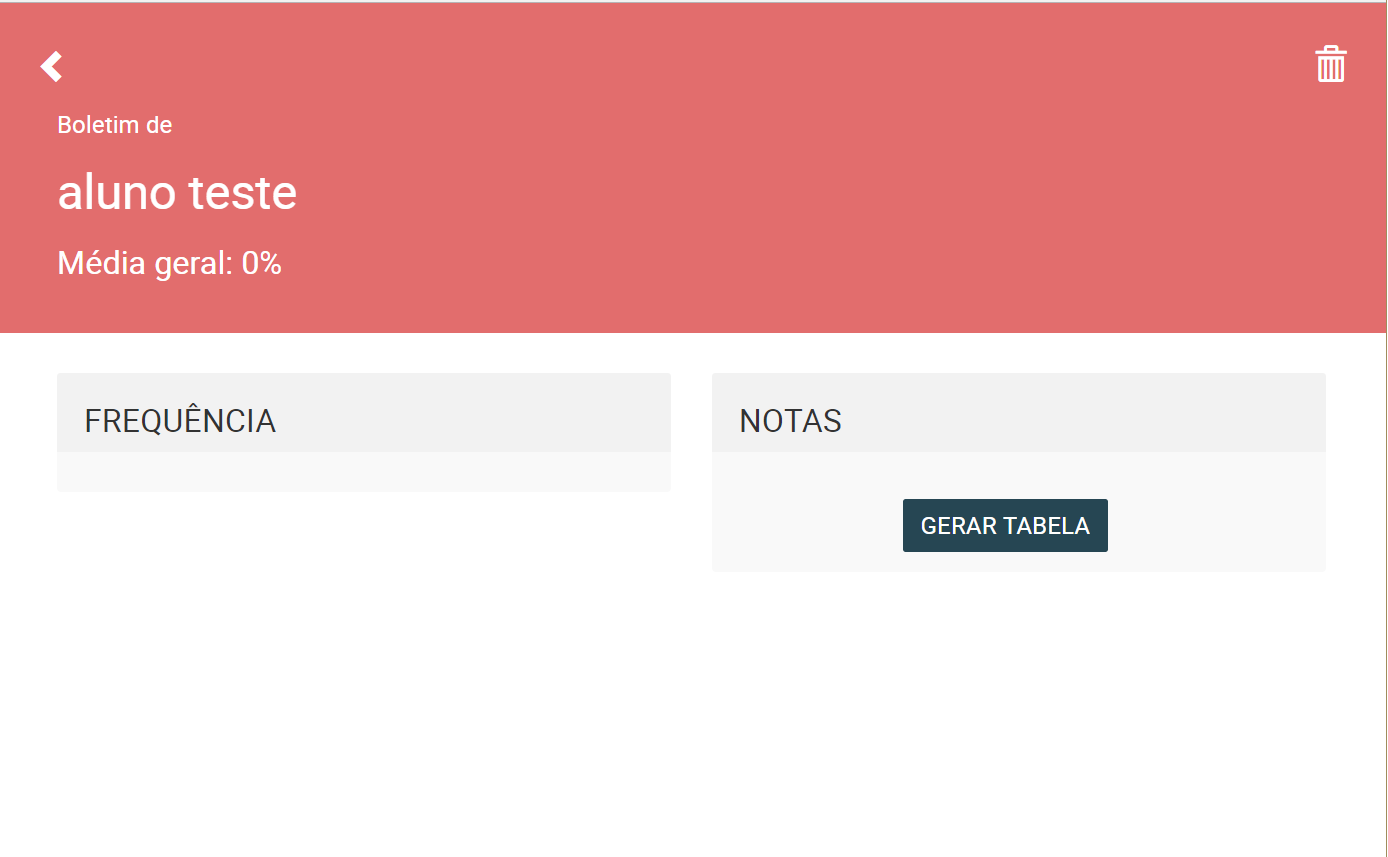
\includegraphics[scale=0.4]{boletimAluno}\\  % 
	{\small } %Fonte da imagem
	\label{boletimAluno} %rotulo para refencia
\end{figure}

\subsection{Aula}

Como parte das funções pedagógicas designadas ao professor, está o registro de aulas. Estas, devem possuir data e, uma descrição curta e objetiva sobre o conteúdo ministrado. Além de qualquer outra ocorrência de importância durante o período da aula.

Também é de responsabilidade do professor, efetuar a chamada, aluno por aluno, e registra-la com presença ou falta.

As funções de editar, cadastrar, excluir e visualizar são implementadas por meio de modais em java script que respondem a chamados da \textit{view}.


%cadastrar aula
\begin{figure}[!htb]
	\centering
	\caption{Cadastro de Aula} %legenda
	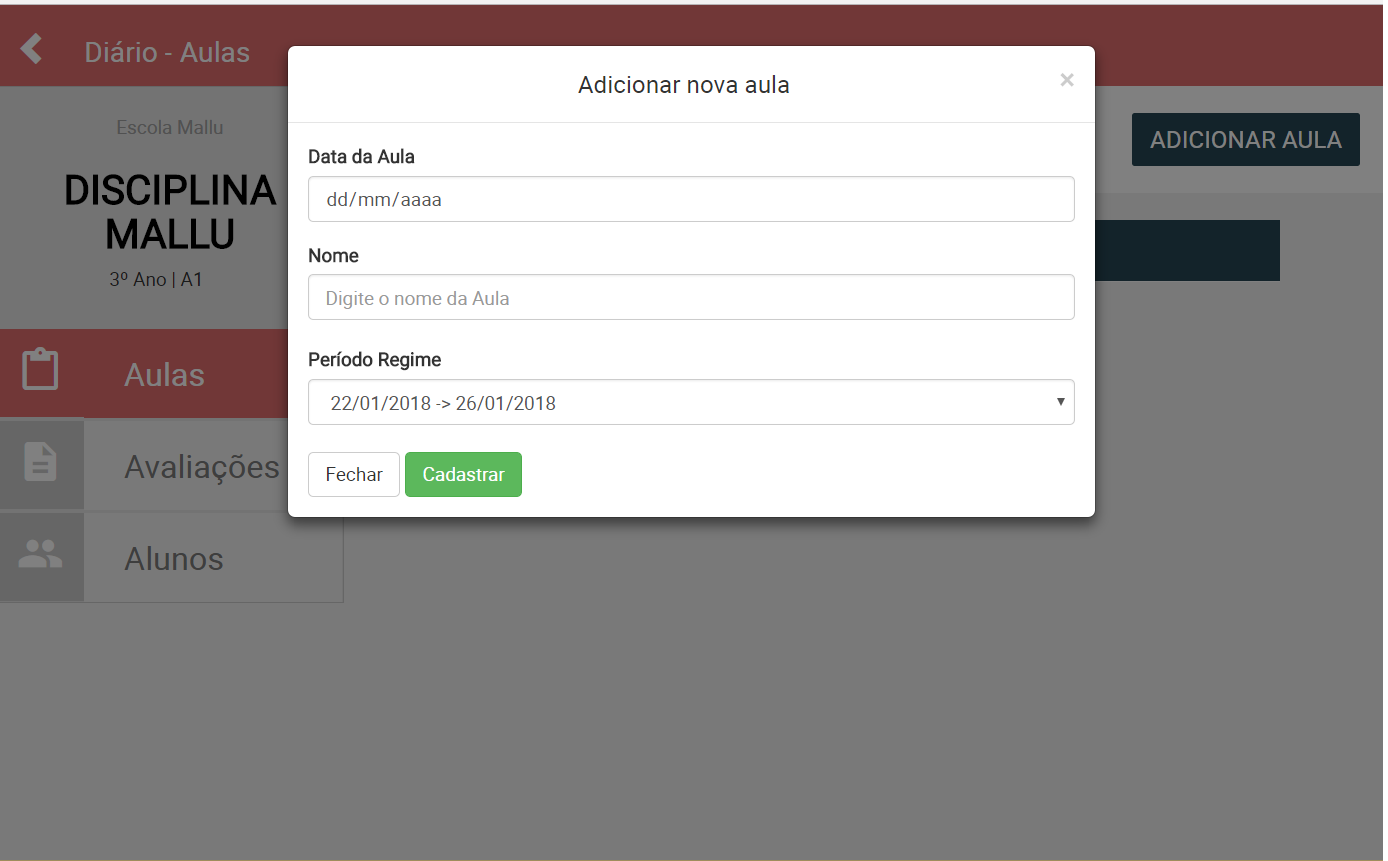
\includegraphics[scale=0.4]{cadastrarAula}\\  % o 
	{\small } %Fonte da imagem
	\label{fig:cadastrarAula} %rotulo para refencia
\end{figure}

%visualizar aulas
\begin{figure}[!htb]
	\centering
	\caption{Visualização das Aulas } %legenda
	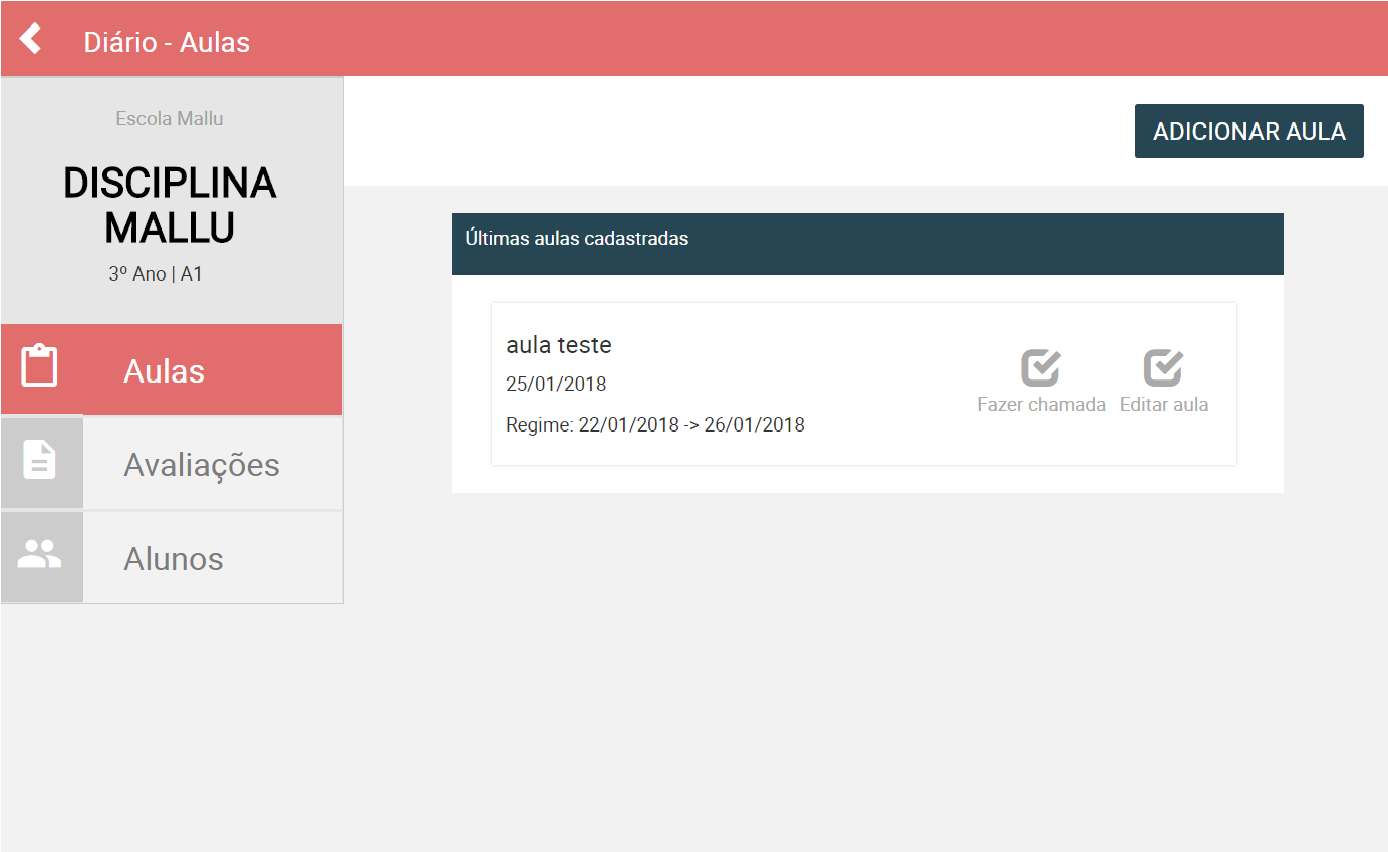
\includegraphics[scale=0.4]{visualizaAulas}\\  % 
	{\small } %Fonte da imagem
	\label{visualizaAulas} %rotulo para refencia
\end{figure}

%presença
\begin{figure}[!htb]
	\centering
	\caption{Listar presença dos Alunos na Aula } %legenda
	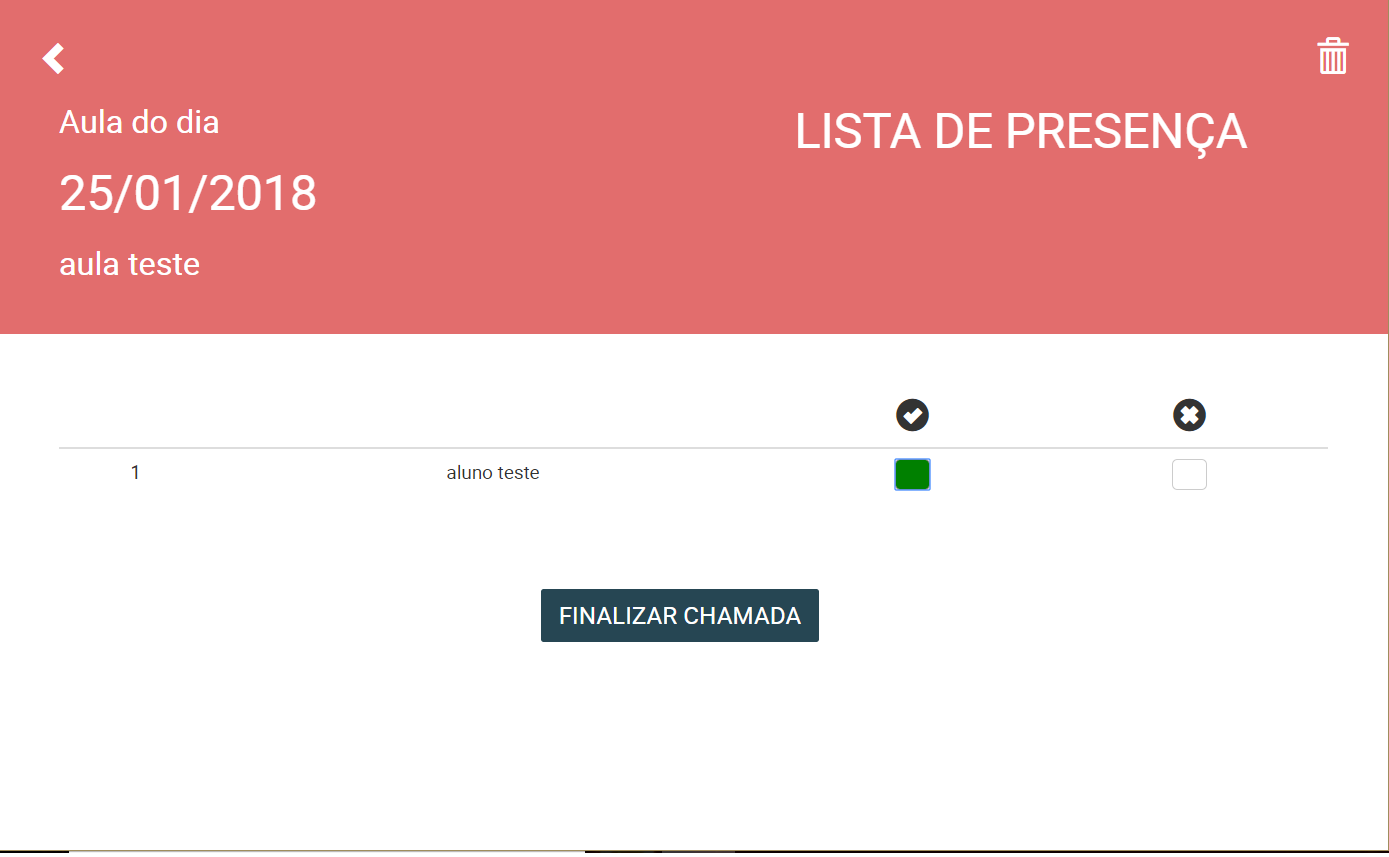
\includegraphics[scale=0.4]{listaPresenca}\\  % 
	{\small } %Fonte da imagem
	\label{listaPresenca} %rotulo para refencia
\end{figure}

\subsection{Avaliação}

Cada período letivo possui um valor. O somatório destes, corresponde ao total de cem pontos no ano letivo e é distribuído em avaliações no decorrer deste. Avaliações são métodos que tem por objetivo dar nota as atividades propostas aos alunos e devem ser registradas no diário pelo professor.

%cadastrar avaliação
\begin{figure}[!htb]
	\centering
	\caption{Cadastro de Avaliacao} %legenda
	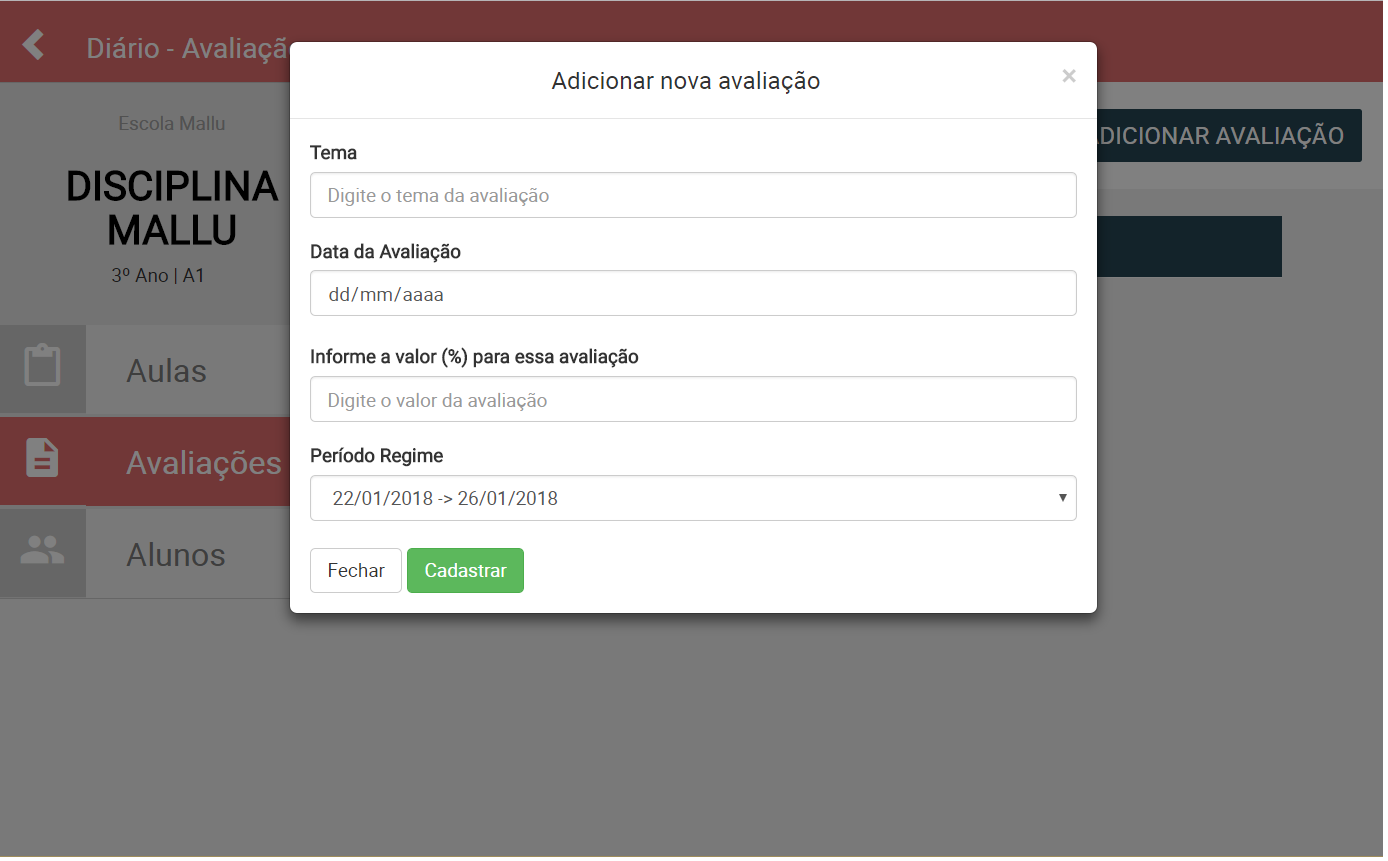
\includegraphics[scale=0.4]{cadastrarAvaliacao}\\ 
	{\small } %Fonte da imagem
	\label{fig:cadastrarAvaliacao} %rotulo para refencia
\end{figure}

%visualizar 
\begin{figure}[!htb]
	\centering
	\caption{Visualização das Avaliações } %legenda
	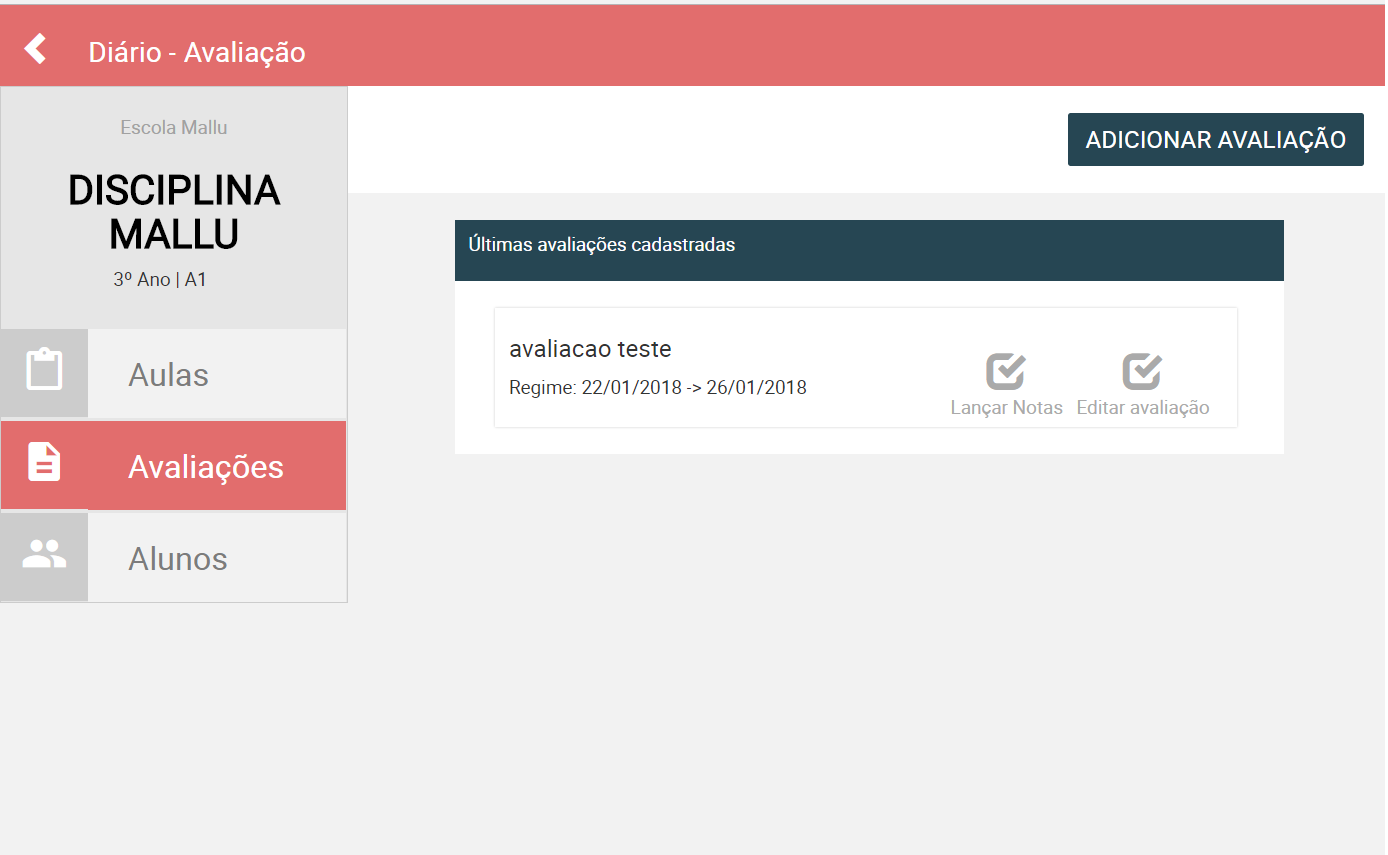
\includegraphics[scale=0.4]{visualizaAvaliacoes}\\  % 
	{\small } %Fonte da imagem
	\label{visualizaAvaliacoes} %rotulo para refencia
\end{figure}

%notas 
\begin{figure}[!htb]
	\centering
	\caption{Lançar nota de Avaliação } %legenda
	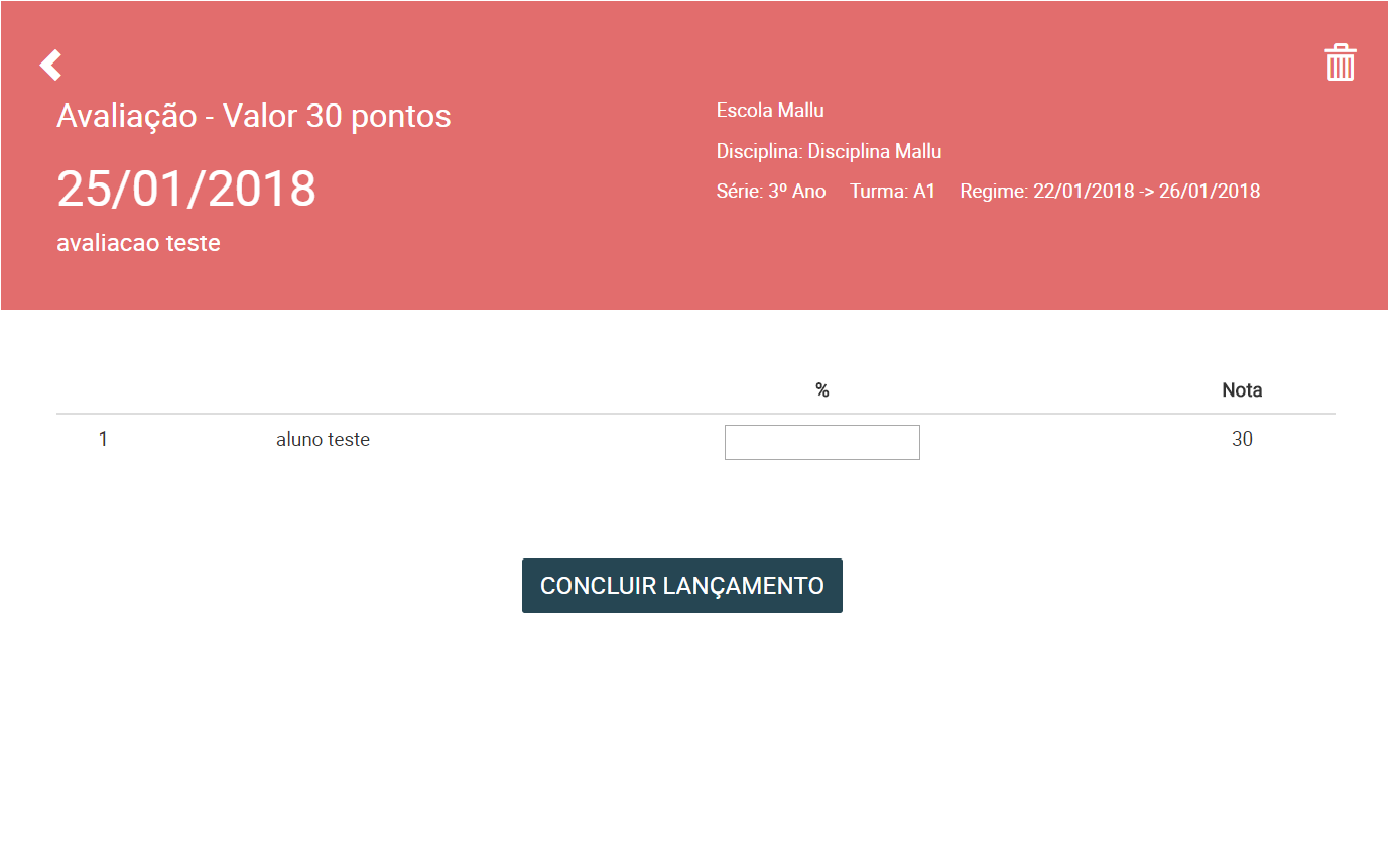
\includegraphics[scale=0.4]{notas}\\  % 
	{\small } %Fonte da imagem
	\label{notas} %rotulo para refencia
\end{figure}
\chapter{CONCLUSÕES}
\label{cap:conclusao}


O módulo proposto para implementação foi desenvolvido e atua como proposta de substituição do Diário de Classe de papel, disponibilizando uma plataforma virtual com os requisitos levantados durante a especificação do projeto.
 É possível acessar a aplicação pelo endereço http://mallusitediario.000webhostapp.com/View/index.php . O código fonte está disponível na plataforma GitHub, pelo endereço:  https://github.com/mallueduardab/ModuloWebDiarioDeClasse.

Como proposta de trabalhos futuros, é interessante a implementação de outros módulos viáveis a integralização da ferramenta com a escola, para auxilio na gestão escolar, como por exemplo, desenvolver os módulos para secretaria e direção.

Ressalta-se também a importância da realização de testes mais completos, com interação dos usuários finais. 

%==============================================================================
% Incluindo bibliografia
%\bibliographystyle{plain}             % estilo para labels em numeros
%\bibliographystyle{alpha}             

\bibliographystyle{abntex2-alf}           % estilo para referências usando ABNT, 
                                       % precisa instalar o abntex para usar!!!

%inclui Referências Bibliográficas
%inclui Referências Bibliográficas
\referencias
\bibliography{relMallu}


%==============================================================================
% Incluindo anexos num1erados com letras maiusculas.
%\anexos
%\include{anexos}


%==============================================================================
% Fim do texto
\end{document}
